%% Energy and AI (Elsevier) submission
%% Migrated from the WileyNJDv5 reviewed version; content unchanged at migration time.
\documentclass[review,times]{elsarticle}

\usepackage{graphicx}
\usepackage{booktabs}
\usepackage{amsmath}
\usepackage{multirow}
\usepackage{array}
\usepackage{tabularx}
\usepackage{url}
\usepackage{siunitx}
\usepackage{xcolor}

\setcounter{secnumdepth}{3}
\graphicspath{{figures/}}

\journal{Energy and AI}

\begin{document}

\begin{frontmatter}

\title{Beyond One-Step Accuracy: Deployment-Oriented Health Prediction for
       Large-Format LiFePO$_4$ Cells\\[2pt]
       {\large Cell-to-Cell Variability, Transfer, and Calibrated Uncertainty}%
       \tnoteref{abbr}}

\tnotetext[abbr]{\textbf{Abbreviations:}
AUC, Area Under the ROC Curve;
BMS, Battery Management System;
CNN, Convolutional Neural Network;
DE, Differential Evolution;
EOL, End of Life;
EV, Electric Vehicle;
FP, Fingerprint;
FT, Fine Tuning;
LFP, Lithium Iron Phosphate;
LCO, Lithium Cobalt Oxide;
LOOCV, Leave-One-Out Cross-Validation;
LSTM, Long Short-Term Memory;
MAE, Mean Absolute Error;
MC, Monte Carlo;
NCA, Nickel Cobalt Aluminium;
NMC, Nickel Manganese Cobalt;
PI, Prediction Interval;
PT, Pretraining;
RMSE, Root Mean Square Error;
RUL, Remaining Useful Life;
SIT, Singapore Institute of Technology;
SOH, State of Health;
ZS, Zero-Shot.}

\author[nu]{Karthickumar Ponnambalam\corref{cor1}}
\ead{K.Ponnambalam2@newcastle.ac.uk}
\author[sit]{Sivaneasan Balakrishnan}
\author[nu]{Anurag Sharma}
\author[nu]{Sze Sing Lee}

\affiliation[nu]{organization={Newcastle University}, country={Singapore}}
\affiliation[sit]{organization={Singapore Institute of Technology}, country={Singapore}}

\cortext[cor1]{Corresponding author.}

\begin{abstract}
Batteries in electric vehicles and grid storage are large-format cells, yet almost
all machine-learning work on battery health is built on small cylindrical cells
cycled in the laboratory, so their transfer to large-format cells is untested. To
close this gap, we release an 18-month dataset of 20 large-format LiFePO$_4$
prismatic cells (50\,Ah) cycled under three operating conditions. The data expose
the core difficulty: manufacturing variability, not temperature or model choice,
dominates how these cells age. Ten nominally identical cells reach final SOH values
that differ by 13.2$\times$ (7.7$\times$ even at the same cycle count), an order of
magnitude wider than any large-format LFP dataset we are aware of; across six
deep-learning models, the individual cell explains 25\% to 58\% of the prediction
error, the model only about 15\%. Can a new cell's health be predicted early,
without months of its own data? Our hybrid model, pretrained on many past cells,
reads a new cell's first 30 cycles through a fingerprint encoder and predicts its
SOH trajectory with no cell-specific training (RMSE 0.025, 38\% better than
training from scratch); fine-tuning raises this to 53.5\% over scratch on all 17
test cells, especially the fast-failing cells that drive warranty risk. It reports
calibrated confidence intervals (94\% coverage, but only
when training and deployment chemistries match), flags defective cells about 50
cycles early (0.78 AUC), and forecasts remaining life to a median of 49 cycles.
Because one-step accuracy saturates, even a linear baseline matches the best, we
judge models by these deployment capabilities and release a reproducible pipeline.

\end{abstract}

\begin{keyword}
battery state of health \sep remaining useful life \sep LiFePO$_4$ \sep
transfer learning \sep cell-to-cell variability \sep uncertainty quantification \sep
large-format cells
\end{keyword}

\end{frontmatter}

\section{Introduction}\label{sec:intro}
The accurate estimation of battery state of health (SOH) is a prerequisite
for the safe and efficient operation of lithium-ion batteries in electric
vehicles (EVs), grid-scale energy storage, and consumer
electronics~\cite{lipu2018review}.
SOH is the ratio of a cell's present usable capacity to its original rated
capacity; as a cell is charged and discharged over hundreds of cycles this
ratio falls, and the point at which it drops too far sets the battery's usable
lifetime and dictates when it must be replaced~\cite{birkl2017degradation}.
Predicting how SOH will decline, ideally early and for each individual cell, is
therefore central to managing cost, safety, and warranty risk in every large
battery deployment.

Over the past decade, deep learning has produced increasingly capable SOH
prediction models, progressing from standard long short-term memory (LSTM)
networks to attention-augmented variants~\cite{qu2019neural} and models whose
hyperparameters are tuned by metaheuristic
search~\cite{ponnambalam2024battery,ponnambalam2026delstm}.
Yet almost all of these methods are developed and benchmarked in the same
narrow setting: small cylindrical 18650 cells of 1 to 3\,Ah (LCO, NMC, or NCA
chemistry) cycled at constant current in the laboratory.
The NASA Prognostics Repository~\cite{saha2007battery}, and in particular its
cells B05, B06, B07, and B18, has been the field's de facto benchmark since
2007, appearing in roughly 30.8\% of all published SOH and remaining-useful-life
(RUL) studies~\cite{xu2025review,bairwa2025cycle}.

This near-exclusive reliance on small laboratory cells creates a gap that only
becomes visible at deployment.
The batteries that actually run electric vehicles and grid storage are
large-format prismatic or pouch cells of 10 to 200\,Ah~\cite{forgez2010thermal},
operated across a wide range of temperatures and charge and discharge rates.
Crucially, cells that are nominally identical, built to the same design on the
same production line, can age very differently because of small, unavoidable
variations introduced during manufacturing~\cite{birkl2017degradation}.
This cell-to-cell variability, of which manufacturing spread is a likely
contributor, is largely absent from the hand-picked, smoothly degrading cells
that populate standard benchmarks, yet it is precisely what a
manufacturer or fleet operator must contend with: warranties, safety margins,
and replacement schedules all depend on predicting the life of each individual
cell, not an average one.
Just how severe this variability is on large-format cells, and whether it,
rather than the choice of algorithm, sets the ultimate limit on prediction,
remains unknown.

A second, more subtle problem lies in how the field measures success.
Almost all of this literature ranks methods by one-step-ahead error: given a
cell's observed history, predict its SOH one cycle into the future.
On the smooth, slowly changing trajectories of large-format cells, however, this
is barely harder than assuming that the next cycle simply repeats the last,
which raises a basic question: can a metric so close to a trivial baseline
actually tell one method apart from another?
If it cannot, then a leaderboard built on it is uninformative, and predictors
need to be judged by something that matters in the field instead, the practical
capabilities they enable: predicting a brand-new cell before it has aged,
attaching trustworthy confidence bounds to each forecast, flagging defective
cells early, and forecasting remaining useful life.

The objective of this paper is to close this gap between benchmark practice and
deployment reality.
Using an 18-month dataset of 20 large-format LiFePO$_4$ prismatic cells
(50\,Ah) cycled under three temperature and C-rate
conditions~\cite{ponnambalam2026sitdata}, we set out to establish how far
cell identity, rather than model choice, governs prediction on
industrial-format cells, and to determine what a prediction method must provide
to be useful once these cells are deployed.
In place of a single accuracy score, we take as our goal a model that can
predict an unseen cell from only its earliest cycles, report and correct its own
uncertainty, remain reliable when the available training data come from a
different battery chemistry, and extend to the related deployment tasks of early
defect screening and remaining-useful-life forecasting.

The remainder of this paper is organised as follows.
Section~\ref{sec:literature} reviews the related literature.
Section~\ref{sec:gap} states the research gaps and summarises the contributions
of this work.
Section~\ref{sec:methodology} describes the datasets, the DE-LSTM baseline, and
the evaluation protocol.
Section~\ref{sec:problem} characterises the deployment challenges empirically on
the SIT cells.
Section~\ref{sec:method} presents the proposed hybrid model.
Section~\ref{sec:results} reports its evaluation, including the ablation study and
the cross-dataset validation.
Section~\ref{sec:screening} shows how the manufacturing-defective cells can be
detected early from the discharge voltage curve.
Section~\ref{sec:rul} extends the hybrid to remaining-useful-life forecasting.
Section~\ref{sec:discussion} discusses implications for deployment, and
Section~\ref{sec:conclusion} concludes.


\section{Literature Review}\label{sec:literature}
This section reviews the prior work most relevant to this study, spanning
SOH prediction methods, large-format and LFP cells, transfer learning,
manufacturing variability, and uncertainty quantification.

\subsection{SOH Prediction Methods}

Data-driven SOH prediction has evolved from simple regression models to
sophisticated deep-learning architectures.
Recurrent neural networks, particularly LSTM variants, have emerged as
the dominant approach due to their ability to model long-range temporal
dependencies in discharge capacity sequences~\cite{zhang2018long}.
Convolutional architectures form a second major family: deep CNNs with
ensemble and transfer learning have been applied to capacity
estimation~\cite{shen2022deep,li2020lithium}, building on early
demonstrations that deep networks can estimate battery state directly from
operational measurements~\cite{chemali2018state}.

Attention mechanisms have been incorporated to allow models to weight
different timesteps in the input window~\cite{bahdanau2015neural}.
Qu et al.\ proposed PA-LSTM, which augments an LSTM encoder with an
attention layer and uses particle swarm optimisation (PSO) for hyperparameter
tuning and model pretraining, with incremental learning for online SOH
monitoring; PA-LSTM outperformed vanilla LSTM, recurrent neural network (RNN), and relevance vector machine (RVM) baselines on
NASA cells~\cite{qu2019neural}.
Subsequent work replaced PSO with other metaheuristics for LSTM hyperparameter
optimisation: genetic algorithm (GA-LSTM)~\cite{ponnambalam2024battery}
and differential evolution~\cite{storn1997differential}
(DE-LSTM)~\cite{ponnambalam2026delstm} both
achieved significant RMSE reductions on the same NASA cells (B05, B06, B18),
retained from PA-LSTM to enable direct comparison.

A common thread across these methods is the use of \textit{incremental
(walk-forward) learning}: the model is trained on the first $p$\% of a cell's
SOH trajectory and evaluated on the remainder, simulating online deployment.
This protocol is adopted throughout the present work.
The proposed hybrid uses the same walk-forward protocol but introduces a
fundamentally different use of early-cycle data: rather than fitting the
observed sequence to continue it, a convolutional encoder summarises the
\textit{shape} of the first 30 cycles into a cell-identity embedding that
initialises the LSTM hidden state before fine tuning begins.
This places each cell in the pretrained population's manufacturing
distribution, discriminating between cell types even when early trajectory
magnitudes appear similar to a sequence-fitting model.

\subsection{Large-Format and LFP Batteries}

Most published SOH prediction studies use 18650-format cylindrical cells
(LCO, NMC, NCA, or LFP chemistry, 1 to 3\,Ah).
Large-format prismatic and pouch cells are the dominant format in stationary
storage and electric heavy vehicles~\cite{barai2015comparison}, yet they
are substantially underrepresented in the prediction literature.
Key differences include: non-uniform current distribution across the
electrode area~\cite{forgez2010thermal}; larger absolute capacity changes
per SOH unit (a 1\% SOH change in a 50\,Ah cell = 0.5\,Ah vs.\ 0.02\,Ah
in a 2\,Ah cell); and different thermal management requirements.

LiFePO$_4$ (LFP) cells are preferred for stationary storage due to their
flat discharge plateau, long cycle life, and superior thermal
stability~\cite{barai2015comparison}.
The flat voltage plateau of LFP makes capacity based SOH estimation more
robust than voltage based methods, motivating the discharge-capacity
incremental learning approach used in this work.

\subsection{Transfer Learning for Battery SOH}

Transfer learning (pretraining a model on a source dataset and adapting
it to a target domain) has attracted growing interest for battery
prognostics~\cite{severson2019data}.
Approaches include fine tuning pretrained networks, domain-adversarial
training, and meta-learning~\cite{finn2017model}.
Yu et al.~\cite{yu2026crossdomain} addressed cross-domain SOH estimation across
heterogeneous small-cell datasets (NASA and CALCE), fusing the most similar
source domains through a similarity network to maintain accuracy when
target-cell data are scarce.
Ye and Yu~\cite{ye2021state} applied domain-adversarial transfer learning to
align feature distributions between source and target cells for SOH estimation.
Closest to the present work, Ma et al.~\cite{ma2022real} achieve personalised,
real-time prediction by fine tuning a pretrained model on each cell's most
recent cycles.
The fingerprint encoder proposed here uses early-life data differently: it
treats the first 30 cycles as a static shape that sets the LSTM initial state
before fine tuning, rather than fine tuning on those cycles directly
(Section~\ref{sec:mechanism}).

A key practical constraint is chemistry: LFP cells have a fundamentally
different degradation mechanism (lithium plating, phase transition stress)
compared to layered-oxide cells such as LiCoO$_2$ (LCO) and NMC (transition metal dissolution, solid electrolyte interphase (SEI) growth)~\cite{birkl2017degradation}.
Whether a model pretrained on one chemistry can transfer to another
is an open question addressed in this work through explicit comparison
of chemistry matched (LFP$\rightarrow$LFP) and chemistry mismatched
(LFP$\rightarrow$LCO) transfer.

\subsection{Manufacturing Variability}

Cell-to-cell variability arising from manufacturing tolerances is
well-documented in the electrochemical literature~\cite{birkl2017degradation}
but rarely quantified in prediction studies.
Dubarry et al.~\cite{dubarry2018synthesize} showed that even cells from
the same batch exhibit measurable differences in electrode loading and
electrolyte fill that propagate to divergent long-term trajectories.
Severson et al.~\cite{severson2019data} observed that early-cycle
statistics (first 100 cycles) correlate with cycle life, motivating
the fingerprint approach adopted here.

To our knowledge, no prior work has simultaneously quantified
manufacturing variability across 10 identical large-format LFP cells
and studied how cross-cell pooling interacts with this variability,
the \textit{two-sided failure mode} we characterise in Section~\ref{sec:variability}.

\subsection{Uncertainty Quantification}

Point-estimate SOH predictions are insufficient for BMS deployment, where
decisions under uncertainty require calibrated prediction intervals.
Bayesian neural networks~\cite{blundell2015weight} and Monte Carlo
Dropout~\cite{gal2016dropout} have been applied to battery SOH uncertainty
estimation~\cite{ke2024bayesian}, but calibration is rarely verified against
held-out data, and never across a chemistry mismatch.
Conformal prediction provides distribution free coverage
guarantees~\cite{angelopoulos2021gentle}, an attractive property for
safety-critical battery management.
In this work we use MC-Dropout and quantify its empirical coverage, revealing
a chemistry-alignment effect in which calibration holds only when the
pretraining and deployment chemistries match.


\section{Research Gap and Contributions}\label{sec:gap}
This section sets out the gaps left open by prior work and summarises how this
study addresses them.

\subsection{Research Gap}

Despite substantial progress in data-driven SOH prediction, three critical gaps remain unaddressed in the existing literature:

\begin{enumerate}
  \item \textbf{Cell-to-cell variability is not modelled.}
        Published benchmarks typically use hand-picked cells with moderate,
        smooth degradation trajectories.
        Cell-to-cell variance, to which manufacturing tolerance is a likely
        contributor, can produce 10$\times$
        differences in degradation rate under identical conditions, is
        systematically understudied.
        Most transfer and fine tuning methods adapt to a target cell either by
        aligning feature distributions across batteries at the population
        level~\cite{ye2021state} or by fine tuning a shared model on the target
        cell's own recent data~\cite{ma2022real}.
        Neither extracts an explicit early-life shape signature that locates a
        cell within the manufacturing distribution of the pretrained population
        before adaptation, so a cell whose early trajectory is ambiguous
        (Section~\ref{sec:variability}) cannot be distinguished from an average
        cell.

  \item \textbf{The standard benchmark protocol has never been validated.}
        Nearly all published comparisons, including our own prior
        work~\cite{ponnambalam2024battery,ponnambalam2026delstm}, rank methods
        by one-step-ahead RMSE on small cylindrical 18650 cells (with NASA cells
        B05, B06, B07, and B18 the de facto standard since
        2007~\cite{saha2007battery,xu2025review}).
        Whether this protocol can actually distinguish methods, that is,
        whether the reported differences exceed trivial-baseline performance
        and the run-to-run variance of training itself, has never been
        tested, and neither has its behaviour on large-format
        ($\geq$10\,Ah) cells under industrially representative conditions.

  \item \textbf{Uncertainty calibration is chemistry-dependent.}
        Bayesian approximations and conformal prediction, including MC-Dropout
        and Bayes by Backprop (BBB), provide well-studied uncertainty
        estimates~\cite{gal2016dropout,angelopoulos2021gentle} and have been
        applied to battery SOH~\cite{ke2024bayesian}, but typically within a
        single chemistry.
        Whether these estimates remain calibrated under a chemistry mismatch
        between pretraining and deployment data has not been investigated, a
        critical gap for practical BMS deployment where pretraining data may be
        available only for a different battery chemistry.
\end{enumerate}

This study addresses these three gaps using the SIT
dataset~\cite{ponnambalam2026sitdata}, our previously published large-format
campaign of 20 LiFePO$_4$ prismatic cells (50\,Ah, 3.2\,V) cycled over 18 months
under three operating conditions. As the baseline we use our previously published
DE-LSTM~\cite{ponnambalam2026delstm}, a differential-evolution-optimised LSTM with
leading accuracy on the NASA 18650 benchmark, alongside five further deep
baselines and two trivial baselines. Section~\ref{sec:problem} quantifies how
severely the first two gaps, cell-to-cell variability and benchmark saturation,
manifest on these cells; Sections~\ref{sec:method} and~\ref{sec:results} present
and validate the proposed hybrid, whose value lies in deployment capabilities
rather than one-step rank; and a cross-dataset evaluation establishes the
chemistry-alignment effect, in which the model's uncertainty estimates stay
calibrated only when pretraining and deployment chemistries match.

\subsection{Contributions}
This paper makes the following key contributions:
\begin{enumerate}
  \item \textbf{Large-format benchmark with trivial-baseline control}: the
        first systematic evaluation of six deep single-cell predictors,
        including our prior DE-LSTM, on 50\,Ah LiFePO$_4$ prismatic cells,
        together with linear-autoregressive and curve-fitting controls that
        expose the saturation of the one-step protocol
        (Section~\ref{sec:baseline}).

  \item \textbf{Cell-to-cell variability quantification}: Across ten nominally
        identical G1 cells, we show that although each cell's own degradation
        trajectory is highly predictable, the cells differ so much from one
        another that this spread between cells, not the algorithm, sets the
        error floor.
        A variance decomposition across six predictors attributes 25\% to 58\%
        of error variance to the cell and only ${\sim}$15\% to the method,
        and cross-cell pooling exhibits a two-sided failure mode: it rescues
        the fast-degrading cells but worsens others by up to 2$\times$
        (Section~\ref{sec:variability}).

  \item \textbf{Benchmark-saturation finding}: We show that the field's
        standard one-step-ahead protocol cannot rank methods on data-rich
        large-format cells: a linear autoregressor attains the lowest error of
        all evaluated models, inter-method differences fall within
        training-run variance, and apparent cross-condition effects are
        dominated by the quality of individual training runs
        (Sections~\ref{sec:baseline} and~\ref{sec:brittleness}).

  \item \textbf{Hybrid transfer model with ablation}: We propose a three-phase
        model (MIT LFP pretraining, convolutional fingerprint encoder,
        MC-Dropout uncertainty) and conduct a full ablation study isolating
        each component's contribution.
        The hybrid predicts new cells from 30 cycles with no target-cell
        fine-tuning (23\% better than scratch) and achieves a 51\%
        mean RMSE improvement over scratch with fine tuning, on all 17 of 17
        test cells; it is the only evaluated method that quantifies
        uncertainty, with prediction intervals that are recalibrated by
        grouped conformal inference (Section~\ref{sec:solution}).
        We additionally characterise pretraining-run variance, show that
        source-domain criteria cannot detect poorly transferring pretraining
        runs, and introduce a calibration-cell checkpoint-selection protocol
        that makes the pipeline reliably reproducible
        (Section~\ref{sec:selection}).

  \item \textbf{Chemistry-alignment effect with multi-dataset validation}:
        We demonstrate that MC-Dropout uncertainty calibration transfers between
        datasets only when pretraining and deployment chemistries are matched
        (LFP$\rightarrow$LFP: 80.8\% coverage; LFP$\rightarrow$LCO: 43.6\%
        coverage).
        A ten-scenario cross-dataset experiment spanning three LFP datasets
        (MIT, SIT, LISHEN 40\,Ah) and one LCO dataset confirms this effect
        and shows that fine tuning is the dependable adaptation mechanism
        across chemistries, while fingerprint conditioning without fine-tuning
        provides its distinctive value before any adaptation is possible, yielding a
        practical guideline for transfer learning in BMS applications
        (Sections~\ref{sec:cross_dataset} and~\ref{sec:discussion}).

  \item \textbf{Early screen for manufacturing-defective cells}: We show that
        no scalar health indicator separates the defective cells within a group,
        yet the early-cycle discharge voltage-curve descriptor $\Delta Q(V)$
        detects eventual early death at an AUC of 0.78 on the SIT cells,
        reproduced on the MIT corpus, about 50 cycles before the capacity
        trajectory reveals the defect (Section~\ref{sec:screening}).

  \item \textbf{Full-coverage probabilistic RUL forecasting}: We extend the
        hybrid from one-step SOH to remaining-useful-life forecasting with a
        direct multi-horizon decoder and a 155-cell multi-dataset LFP foundation
        corpus, forecasting every cell that reaches end of life, including the
        catastrophic cells that recursive baselines abstain on, at a median
        error of 49 cycles at the midlife anchor with conformally calibrated
        intervals (Section~\ref{sec:rul}).
\end{enumerate}


\section{Dataset and Experimental Methodology}\label{sec:methodology}
This section describes the datasets used in this study, the DE-LSTM baseline
against which the hybrid is developed, and the evaluation protocol shared by all
experiments.

\subsection{Datasets}\label{sec:datasets}

\subsubsection{SIT LiFePO$_4$ Dataset (Primary)}
The SIT dataset~\cite{ponnambalam2026sitdata} comprises 20 commercial
LiFePO$_4$ prismatic cells (Narada Power Source, 50\,Ah nominal, 3.2\,V)
cycled in the Singapore Institute of Technology Battery Laboratory over
18 months.
Cells are organised into three groups differing in temperature and C-rate:
\begin{itemize}
  \item \textbf{G1} (10 cells, IDs 001-1 to 001-8, 101-1, 101-3):
        ambient temperature (${\approx}25$\,\textcelsius), 1\,C charge/discharge,
        deep cycling. All cells share nominally identical specifications
        and protocol, so observed differences are most plausibly dominated by
        manufacturing tolerances, although cycler-channel differences, contact
        resistance, minor temperature variation, testing interruptions and
        production batch may also contribute.
  \item \textbf{G2} (4 cells, IDs 002-1 to 002-4):
        40\,\textcelsius\ thermal chamber, 1\,C rate.
  \item \textbf{G3} (6 cells, IDs 002-5, 002-7, 003-1, 003-3, 003-5, 003-7):
        40\,\textcelsius\ thermal chamber, 2\,C rate.
\end{itemize}
SOH is computed from discharge capacity as
$\text{SOH}(k) = Q_k / Q_1$,
where $Q_k$ is discharge capacity at cycle $k$ and $Q_1$ is the first-cycle
capacity.
Table~\ref{tab:sit_cells} summarises cycle counts and final SOH for all
20 cells, where SOH$_\text{end}$ is the final-cycle SOH.
Cell 003-5 records SOH$>$1, a capacity-recovery artefact arising at low C-rate
after elevated-temperature cycling; it is retained in the analysis but treated
with caution.

\begin{table}[pos=htbp]
\caption{SIT cell inventory across three operating conditions.}
\label{tab:sit_cells}
\resizebox{\columnwidth}{!}{%
\begin{tabular}{llrrr}
\toprule
Group & Cell & Cycles & SOH$_\text{end}$ & Condition \\
\midrule
G1 & 001-1 & 876  & 0.767 & \multirow{10}{*}{25\,\textcelsius, 1\,C} \\
   & 001-2 & 764  & 0.878 & \\
   & 001-3 & 788  & 0.493 & \\
   & 001-4 & 878  & 0.709 & \\
   & 001-5 & 684  & 0.885 & \\
   & 001-6 & 876  & 0.854 & \\
   & 001-7 & 876  & 0.885 & \\
   & 001-8 & 764  & 0.067 & \\
   & 101-1 & 864  & 0.696 & \\
   & 101-3 & 697  & 0.118 & \\
\midrule
G2 & 002-1 & 564  & 0.924 & \multirow{4}{*}{40\,\textcelsius, 1\,C} \\
   & 002-2 & 572  & 0.888 & \\
   & 002-3 & 561  & 0.915 & \\
   & 002-4 & 560  & 0.660 & \\
\midrule
G3 & 002-5 & 689  & 0.913 & \multirow{6}{*}{40\,\textcelsius, 2\,C} \\
   & 002-7 & 695  & 0.564 & \\
   & 003-1 & 603  & 0.461 & \\
   & 003-3 & 693  & 0.559 & \\
   & 003-5 & 567  & 1.075$^\dagger$ & \\
   & 003-7 & 694  & 0.587 & \\
\bottomrule
\multicolumn{5}{l}{$\dagger$ Capacity recovery artefact; included in analysis with caution.}
\end{tabular}%
}
\end{table}

G1 provides the cell-to-cell variability experiment (Section~\ref{sec:variability});
G1/G2/G3 provide the cross-condition transfer experiment
(Section~\ref{sec:brittleness}).

\subsubsection{MIT LFP Dataset (Pretraining)}
The Severson et al.~\cite{severson2019data} dataset provides 124 LFP/graphite
18650 cells (1.1\,Ah) cycled at Stanford University and Toyota Research
Institute at various C-rates and charging protocols.
Of these, 49 cells have complete cycle-level capacity data in our processing;
the \emph{pretraining corpus} comprises the 40 batch-1 cells
(batch1\_cell000 to 039).
This choice is empirical: in a corpus-sensitivity test, extending the corpus
with the nine remaining complete-data cells (including the two batch-3 cells
with $\leq$9\% total fade) collapsed the next-cycle pretraining objective
toward a trivial persistence solution (validation MSE
$3.4\times10^{-3}\rightarrow1\times10^{-5}$) and degraded downstream transfer;
the 40-cell corpus is therefore retained, and the full corpus-sensitivity
results are provided in the released repository.
We emphasise that this is a property of the pretraining objective, not a
fragility of the deployed model: the hybrid is evaluated on, and performs well
on, slowly fading target cells (e.g.\ the G2 cells with final SOH
${\approx}0.9$).
The early-life correlation analysis of Table~\ref{tab:fingerprint} uses the
47 genuine degraders (final SOH $<1$) among all 49 complete-data cells,
excluding the two capacity-recovery artefacts.
Pretraining on chemistry matched LFP cells is a deliberate design choice
motivated by the chemistry and domain alignment effect evaluated in
Section~\ref{sec:discussion}.

\subsubsection{External Datasets}
Four further datasets support the cross-chemistry test and the transfer and RUL
experiments. The NASA Prognostics Center of Excellence
dataset~\cite{saha2007battery} provides 26 lithium cobalt oxide (LCO) 18650
cells of about 2\,Ah cycled at several ambient temperatures under
constant-current discharge; because its chemistry differs from the LFP target
cells, it serves as the cross-chemistry generalisation test. The LISHEN
dataset~\cite{lishen_zenodo} provides 3 large-format 40\,Ah LFP prismatic cells
cycled at 2\,C over a 20\% depth-of-discharge window, used as a third,
independent LFP source in the cross-dataset transfer matrix. The HUST~\cite{ma2022real} and Sandia
(SNL)~\cite{preger2020degradation} collections provide 77 and 29 LFP 18650 cells respectively; together with
the 49 MIT cells they form the 155-cell LFP foundation corpus that pretrains the
RUL decoder (Section~\ref{sec:rul_foundation}). Table~\ref{tab:datasets}
consolidates the chemistry, format, capacity, cell count, operating conditions,
and role of every dataset used in this study.

\begin{table*}[pos=tbp]
\centering
\caption{Datasets used in this study.}\label{tab:datasets}
\footnotesize
\resizebox{\textwidth}{!}{%
\begin{tabular}{l l l r r l l}
\toprule
Dataset & Chemistry & Format & Cap.\ (Ah) & Cells & Conditions & Role in this study \\
\midrule
SIT (primary)~\cite{ponnambalam2026sitdata} & LFP & Prismatic & 50  & 20 & 25 to 40\,\textcelsius, 1 to 2\,C     & Target cells: testing and checkpoint selection \\
MIT/Severson~\cite{severson2019data}  & LFP & 18650     & 1.1 & 40 & Fast charge, multi-protocol           & Base-hybrid pretraining (training) \\
NASA PCoE~\cite{saha2007battery}     & LCO & 18650     & 2   & 26 & Varied temperature, constant current  & Cross-chemistry test (testing) \\
LISHEN~\cite{lishen_zenodo}        & LFP & Prismatic & 40  & 3  & 2\,C, 20\% depth of discharge         & Third LFP source, cross-dataset transfer \\
HUST~\cite{ma2022real}          & LFP & 18650     & 1.1 & 77 & Multi-rate discharge                  & RUL foundation corpus (training) \\
SNL (Sandia)~\cite{preger2020degradation}  & LFP & 18650     & 1.1 & 29 & Varied temperature, rate, DOD         & RUL foundation corpus (training) \\
\bottomrule
\end{tabular}%
}
\end{table*}

\subsection{Baseline: DE-LSTM}\label{sec:delstm}

DE-LSTM~\cite{ponnambalam2026delstm} is the strongest model from our prior work
and serves as the baseline against which the hybrid is developed.
It is a plain LSTM network whose
hyperparameters (hidden units $H$, look-back window $W$,
learning rate $\eta$) are optimised by differential
evolution (DE)~\cite{storn1997differential} using
2-fold walk-forward cross-validation as the fitness function;
the batch size is set deterministically to $\max(32, H)$ rather than searched.
The architecture is:
\begin{equation}
  \hat{y}_t = \mathbf{W}_o\, h_t + b_o,\quad
  h_t, c_t = \mathrm{LSTM}(x_{t-W:t},\, h_{t-1}, c_{t-1})
\end{equation}
where $x_{t-W:t}$ is the SOH look-back window of length $W$, $h_t$ and $c_t$ are
the LSTM hidden and cell states at cycle $t$, $\mathbf{W}_o$ and $b_o$ are the
output-layer weight matrix and bias, and $\hat{y}_t$ is the predicted next-cycle
SOH.

For the SIT baseline evaluation (Section~\ref{sec:baseline}), DE is run
independently for each cell and each training split, with the search space
$H \in \{8, 16, 32, 64, 128, 256\}$, $W \in [3, 30]$, $\eta \in [10^{-4}, 0.05]$.
The DE search uses a population of 3 per parameter and a maximum of
8 generations (\texttt{polish=False}, \texttt{tol}~$=10^{-4}$), on the order of
80 candidate evaluations per cell and split, and is itself run under a single
fixed seed.
The selected hyperparameters are then re-evaluated under two independent random
seeds, and the mean RMSE is reported.

\subsection{Evaluation Protocol}\label{sec:eval}

All experiments use three training splits: 30\%, 50\%, and 70\% of each
cell's SOH trajectory, with the remainder held out for evaluation.
Because each split is defined as a fraction of a cell's already-completed
trajectory, these splits are retrospective (they presuppose the cell's total
lifetime). Prediction is performed in a rolling one-step-ahead manner: at each
held-out cycle the model receives the \emph{observed} previous $W$ SOH values and
predicts the next one, and predicted values are never fed back as inputs (i.e.,
we report one-step-ahead prediction, not recursive multi-step forecasting).
Hybrid-model evaluations are averaged over five random seeds per cell;
single-cell baseline methods (Simple, PA-, GA-, DE-LSTM, TCN, Transformer)
are averaged over two seeds after their hyperparameter search, which itself
runs under a single fixed seed.
Summary tables report the mean RMSE with its
standard deviation across the cells in each group.
Improvement over scratch LSTM is computed per cell and then averaged, so a
reported improvement is the mean of the per-cell percentage RMSE reductions rather
than the percentage change between the group-mean RMSEs.

\subsubsection{Data Partitioning and Leakage}
Within each target cell the training and evaluation partitions are contiguous in
cycle order: training windows are drawn from the first $p\%$ of the trajectory and
evaluation windows from the remainder, so no held-out SOH value is ever used as a
training target. The first evaluation window is seeded with the last $W$
\emph{observed} training cycles as its input; this is inherent to one-step-ahead
prediction and exposes no held-out target. For pretraining, the look-back windows
of all corpus cells are pooled in cell order and the final 10\% of the pooled array
is held out for early stopping. Because the pooled array is not shuffled before
this split, the validation slice comprises whole cells except for the single cell
straddling the boundary, which is consequently the only cell able to contribute
(mutually overlapping) windows to both partitions. Finally, since a cell of length
$T$ yields $T-W$ windows, cells with longer trajectories contribute proportionally
more pretraining samples: the pooled corpus is sample-weighted by trajectory
length rather than balanced per cell.

\subsubsection{Calibration Cells and Test Cells}
Three SIT cells, the numerically first cell of each condition group
(001-1, 002-1, 002-5), designated \emph{a priori}, are reserved as
\emph{calibration cells} for pretraining-checkpoint selection
(Section~\ref{sec:selection}).
All reported SIT results are computed on the remaining \textbf{17 test cells};
the calibration cells never contribute to any reported metric.

\subsubsection{Reproducibility}
All experiments run with deterministic GPU kernels
(TensorFlow op-determinism, full float32) and complete seeding of the Python,
NumPy, and TensorFlow generators, so every reported number is bit-for-bit
reproducible on the same hardware and software stack.
The code, the full pipeline, and the selected pretrained checkpoint are
permanently archived on Zenodo~\cite{ponnambalam2026code}.
Statistical significance of pairwise comparisons uses the Wilcoxon
signed-rank test~\cite{wilcoxon1945individual} at $\alpha = 0.05$.
This non-parametric test is preferred over a paired $t$-test because
per-cell RMSE distributions are skewed by outlier cells (e.g., catastrophic
degraders such as cell 001-8), and the Wilcoxon test does not assume normality.
For the hybrid model, empirical 95\% prediction-interval (PI) coverage (fraction
of test points within the predicted interval) and mean PI width are additionally
reported. These MC-Dropout intervals are approximate prediction intervals, not
calibrated prediction intervals in the conformal sense.

\subsubsection{Model Configurations and Tuning Budget}
Table~\ref{tab:hyperparams} reports every model's architecture, tuning budget, and
training configuration exactly as run. The three search-based LSTMs (PA-, GA- and
DE-LSTM) each receive a per-cell, per-split hyperparameter search of comparable
size (of the order of 80 candidate evaluations), whereas the Simple LSTM, the TCN
and the Transformer share a common fixed configuration. We note this asymmetry
explicitly: the non-recurrent baselines are not hyperparameter-optimised, so their
weaker performance should be read as evidence that a richer backbone is not what
these data reward rather than as a tuned upper bound. The proposed hybrid likewise
receives \emph{no} per-cell search, and so competes against the searched LSTM
baselines from a single fixed configuration.

\begin{table*}[pos=tbp]
\caption{Model configurations and training budgets, as run (per cell and split).}
\label{tab:hyperparams}
\centering
\footnotesize
\begin{tabularx}{\textwidth}{l X l X}
\toprule
Model & Architecture & Tuning budget & Training configuration \\
\midrule
Simple LSTM & LSTM(64) $\to$ Dense(1) & none (fixed) & $W{=}20$, $\eta{=}10^{-2}$, batch 64, 200 epochs, early stop patience 10 \\
PA-LSTM & LSTM $\to$ attention $\to$ pooling $\to$ Dense(1) & PSO, ${\approx}80$ evals & searched: $H\in\{8\ldots256\}$, $W\in[3,30]$, $\eta\in[10^{-4},5{\times}10^{-2}]$; batch $\max(32,H)$, 200 epochs, patience 10 \\
GA-LSTM & LSTM $\to$ Dense(1) & GA, $9{\times}9$ evals & searched, as PA-LSTM \\
DE-LSTM & LSTM $\to$ Dense(1) & DE, ${\approx}80$ evals & searched, as PA-LSTM \\
TCN & 3 residual dilated causal conv blocks (64 filters, $k{=}3$, dilations $1,2,4$) & none (fixed) & $W{=}20$, $\eta{=}10^{-2}$, batch 64, 200 epochs, patience 10 \\
Transformer & 1 encoder block ($d_{\mathrm{model}}{=}64$, 4 heads, feed-forward 128) & none (fixed) & $W{=}20$, $\eta{=}10^{-3}$, batch 64, 200 epochs, patience 10 \\
\midrule
Scratch LSTM & LSTM(64) $\to$ Dropout(0.2) $\to$ Dense(1) & none (fixed) & $W{=}20$, $\eta{=}10^{-3}$, 100 epochs, patience 10 \\
Hybrid (ours) & CNN fingerprint (Conv1D 32 and 16, $k{=}3$, global average pooling, Dense 16) $\to$ LSTM(64) initialised with $(h_0,c_0)$ $\to$ MC-Dropout(0.2) $\to$ Dense(1); 21\,089 parameters & none (fixed) & pretrain: $\eta{=}10^{-3}$, batch 64, 100 epochs, patience 12; fine tune: $\eta{=}5{\times}10^{-4}$, 50 epochs, patience 8; 50 MC-Dropout passes \\
\bottomrule
\end{tabularx}
\end{table*}


\section{Problem Characterisation: Limitations of Standard Methods}\label{sec:problem}
Before introducing the hybrid model, we use the SIT cells to characterise the
problem landscape: we establish the DE-LSTM baseline, show that the standard
one-step evaluation protocol saturates on these data, quantify the
cell-to-cell variability that limits pooled prediction, and examine how
training-run variance confounds cross-condition comparisons.

\subsection{Baseline Performance on the SIT Cells}\label{sec:baseline}

Figure~\ref{fig:sit_overview} shows the SOH trajectories for all 20 cells.
Within G1 (identical conditions), final SOH spans 0.067 to 0.885 (a
13.2$\times$ ratio), illustrating the scale of cell-to-cell variability.
G2 cells (elevated temperature) show consistently high residual SOH
(0.660 to 0.924), suggesting the 40\,\textcelsius\ chamber protocol did not
accelerate degradation within the test duration.
G3 cells (elevated temperature and 2C rate) show more diverse outcomes
(0.461 to 1.075), including two cells with moderate to severe degradation.

\begin{figure*}[htbp]
\centering
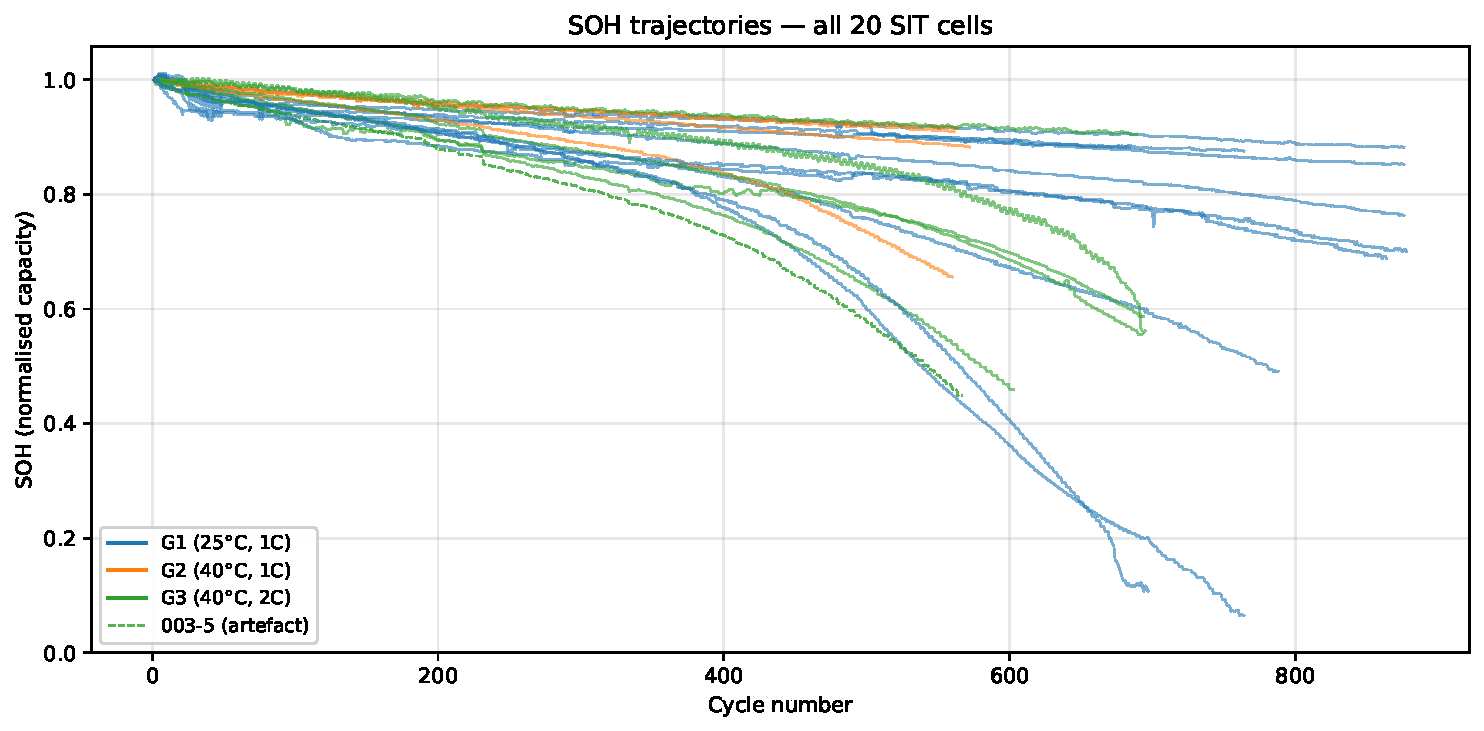
\includegraphics[width=\textwidth]{fig2_sit_overview}
\caption{SOH trajectories for all 20 SIT cells.}
\label{fig:sit_overview}
\end{figure*}

Table~\ref{tab:sit_baseline} reports DE-LSTM RMSE across all 20 SIT cells
at 30\%, 50\%, and 70\% training splits; values are mean\,$\pm$\,std across the
cells in each group, averaged over two evaluation seeds.

\begin{table}[htbp]
\caption{DE-LSTM baseline RMSE by operating-condition group.}
\label{tab:sit_baseline}
\footnotesize
\begin{tabular*}{\columnwidth}{@{\extracolsep{\fill}}llrrr}
\toprule
Group & Condition & RMSE (30\%) & RMSE (50\%) & RMSE (70\%) \\
\midrule
G1 & 25\,\textcelsius, 1C & $0.030\pm0.025$ & $0.012\pm0.005$ & $0.010\pm0.006$ \\
G2 & 40\,\textcelsius, 1C & $0.018\pm0.021$ & $0.011\pm0.007$ & $0.011\pm0.008$ \\
G3$^\dagger$ & 40\,\textcelsius, 2C & $0.020\pm0.021$ & $0.011\pm0.008$ & $0.010\pm0.008$ \\
\midrule
All$^\dagger$ & {}                   & $0.025\pm0.023$ & $0.011\pm0.006$ & $0.010\pm0.007$ \\
\bottomrule
\multicolumn{5}{@{}l}{\footnotesize $^\dagger$ Excluding the recovery-artefact cell 003-5, whose 30\%-split}\\
\multicolumn{5}{@{}l}{\footnotesize RMSE (0.234) is dominated by its SOH$>$1 segment (50/70\%: 0.017/0.014).}
\end{tabular*}
\end{table}

Two patterns are immediately evident.
First, within G1, per-cell RMSE still varies ${\sim}5\times$ (0.004 to 0.021
at the 50\% split) despite identical conditions
(Figure~\ref{fig:sit_baseline_percell}), and the worst cells at every split
are the catastrophic degraders and the recovery artefact, whose early history
is unrepresentative of their future.
Second, once half a cell's history is available the per-cell errors are small
(${\sim}$0.01) and nearly uniform across operating conditions, a first hint
that the one-step task itself is close to its floor, which the next comparison
makes explicit.

\begin{figure}[htbp]
\centering
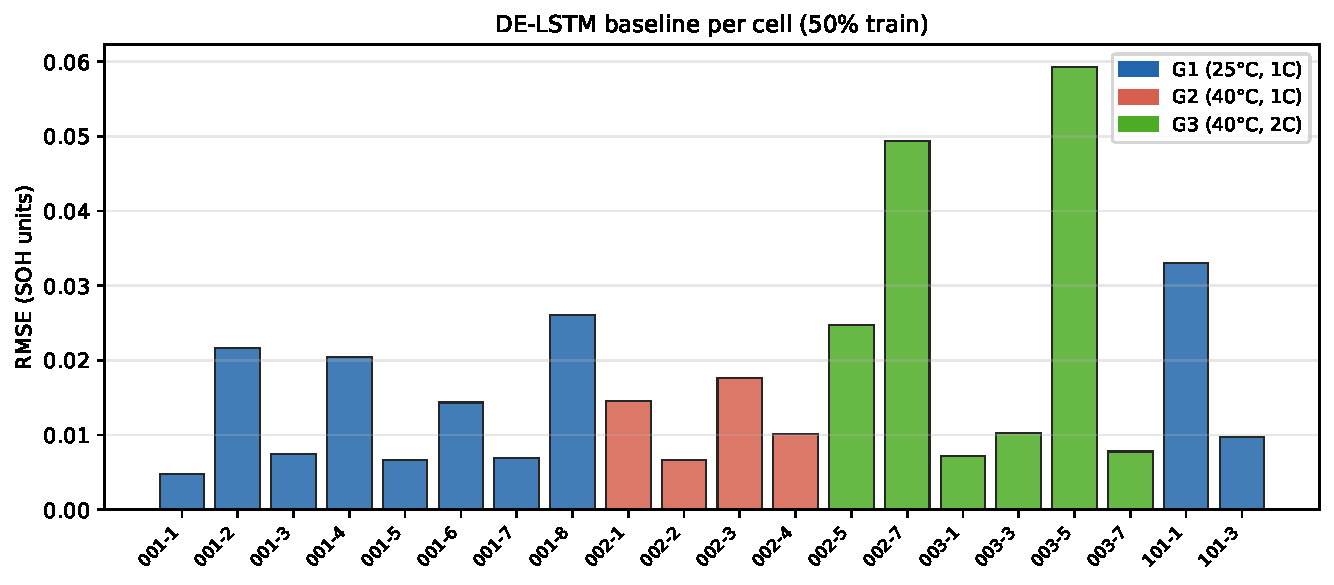
\includegraphics[width=\columnwidth]{fig3_sit_baseline}
\caption{DE-LSTM per-cell RMSE at the 50\% split for all 20 SIT cells, sorted by
final SOH.}
\label{fig:sit_baseline_percell}
\end{figure}

\subsubsection{Comparison with Established Methods}

To confirm that this error floor reflects the dataset rather than a weakness of
DE-LSTM specifically, we compare six single-cell predictors on the
17 test cells under the identical protocol: four LSTM-family methods (a
fixed-hyperparameter Simple LSTM, the attention-based
PA-LSTM~\cite{qu2019neural}, GA-LSTM~\cite{ponnambalam2024battery},
and DE-LSTM~\cite{ponnambalam2026delstm}) and two modern non-recurrent
architectures: a temporal convolutional network (TCN, dilated causal
convolutions) and a Transformer encoder, each under a fixed configuration
matched to the Simple-LSTM protocol.
Table~\ref{tab:method_comparison} reports the mean RMSE over the test cells at each split.

\begin{table}[htbp]
\caption{Single-cell predictor and trivial-baseline RMSE on the SIT test cells.}
\label{tab:method_comparison}
\footnotesize
\begin{tabular*}{\columnwidth}{@{\extracolsep{\fill}}lrrr}
\toprule
Method & RMSE (30\%) & RMSE (50\%) & RMSE (70\%) \\
\midrule
\multicolumn{4}{@{}l}{\textit{Recurrent (LSTM family)}} \\
Simple LSTM & $0.0661$ & $0.0352$ & $0.0239$ \\
PA-LSTM~\cite{qu2019neural} & $0.0158$ & $0.0263$ & $0.0173$ \\
GA-LSTM~\cite{ponnambalam2024battery} & $0.0633$ & $0.0198$ & $0.0122$ \\
DE-LSTM~\cite{ponnambalam2026delstm} & $0.0379$ & $0.0118$ & $0.0105$ \\
\midrule
\multicolumn{4}{@{}l}{\textit{Non-recurrent (modern)}} \\
TCN         & $0.1078$ & $0.1017$ & $0.1089$ \\
Transformer & $0.1681$ & $0.1130$ & $0.1001$ \\
\midrule
\multicolumn{4}{@{}l}{\textit{Trivial baselines}} \\
Persistence ($\hat{y}_t=y_{t-1}$) & $0.0123$ & $0.0128$ & $0.0134$ \\
Drift ($\hat{y}_t=2y_{t-1}-y_{t-2}$) & $0.0210$ & $0.0219$ & $0.0228$ \\
Linear AR & $\mathbf{0.0068}$ & $\mathbf{0.0052}$ & $\mathbf{0.0052}$ \\
Cubic curve fit & $1.499$ & $0.158$ & $0.088$ \\
\bottomrule
\end{tabular*}
\end{table}

\begin{figure}[htbp]
\centering
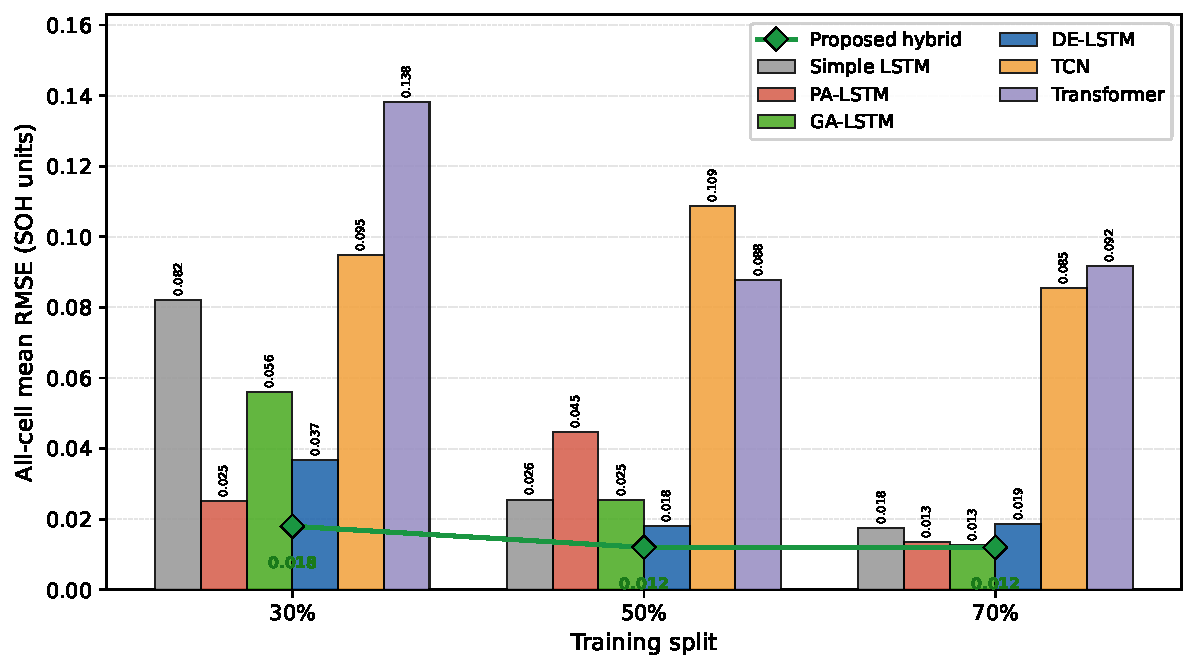
\includegraphics[width=\columnwidth]{fig_method_comparison}
\caption{Mean RMSE of six single-cell predictors and the proposed hybrid across the 30\%, 50\% and 70\% splits.}
\label{fig:method_comparison}
\end{figure}

Table~\ref{tab:method_comparison} shows that the one-step protocol is
saturated on these data: a \textbf{20-cycle linear autoregressor attains the
lowest error at every split}, on par with or ahead of all six deep models, and
even a \textbf{memoryless persistence predictor} ($\hat{y}_t=y_{t-1}$, RMSE
0.013 at 50\%) matches the best deep model (DE-LSTM, 0.0118) and beats the
proposed hybrid (0.0156) on this metric. Among the deep models themselves no
consistent ranking emerges (PA-LSTM leads at
30\%, DE-LSTM at 50\% and 70\%, in sharp contrast to the NASA benchmark where
DE-LSTM reduces RMSE by \mbox{85 to 91\%} over PA-LSTM and
GA-LSTM~\cite{ponnambalam2026delstm}).
This is a property of the task rather than a weakness of any one model, and it
is precisely why, on large-format cells, a predictor must be judged by the
capabilities it provides rather than by its one-step rank, the case the rest of
this paper makes for the proposed hybrid.
The explanation is that rolling one-step-ahead prediction from \emph{observed}
windows is a near-persistence task on smooth SOH trajectories: successive
cycles differ by a fraction of a percent, the predictor always receives the
true recent history, and a linear map over the last 20 observations is
essentially optimal.
The task never requires anticipating a knee or a crash, only following one
cycle behind it, which is also why the curve-fitting baseline, the one
trivial method forced to extrapolate, fails by an order of magnitude.
We term this \textbf{benchmark saturation}: the protocol under which this
method lineage, and much of the field, ranks models cannot in fact
distinguish them.
A two-way variance decomposition over the six deep predictors makes the point
quantitatively: the identity of the \emph{cell} explains 58\%/31\%/25\% of
prediction-error variance at the 30/50/70\% splits respectively, whereas the
choice of \emph{method} explains only 15\% to 17\% at every split, with the
remainder attributable to cell-method interaction and training-run variance.
Model selection should therefore rest not on one-step leaderboards but on
capabilities the task actually demands: predicting cells with \emph{no}
usable history, quantifying uncertainty honestly, and transferring across
operating regimes and chemistries, the capabilities evaluated in
Section~\ref{sec:results}.

\subsection{Cell-to-Cell Variability and the Two-Sided Failure Mode}\label{sec:variability}

We examine this cell-to-cell variability from three angles: how predictable each
cell is on its own, what happens when a model is pooled across cells, and whether
early-life data can identify the problem cells in advance.

\subsubsection{Variability at Matched Exposure}
The 13.2$\times$ spread in final SOH (0.067 to 0.885) compares cells at different
points in their lives, because they reach end of life after different cycle counts.
To measure the variability fairly we compare the G1 cells at matched exposure. At a
common cycle count, the shortest G1 record of 684 cycles, SOH ranges from 0.20 to
0.90, a 7.6$\times$ ratio; at a common cumulative discharge throughput of
26.8\,kAh it ranges from 0.07 to 0.92, a 13.7$\times$ ratio. The spread therefore
remains roughly 8 to 14 times under every matched-exposure definition, so it is not
an artefact of unequal test durations but a genuine dispersion among
nominally identical cells.

\subsubsection{Within-Cell Predictability}

A cubic polynomial fit to each G1 cell's SOH trajectory achieves a mean
$R^2$ of 0.964 (minimum: 0.908 for cell 001-6), confirming that individual
trajectories are highly predictable given sufficient training data.
On average 3.6\% of the trajectory variation is not captured by this
particular cubic fit; this residual reflects the choice of fit and is not
an irreducible noise floor.
The challenge is therefore not within-cell prediction but
\textit{between-cell diversity}: knowing a cell's past trajectory does not
reveal where it sits in the manufacturing distribution.

\subsubsection{Cross-Cell LOOCV: A Two-Sided Failure Mode}

\begin{figure*}[htbp]
\centering
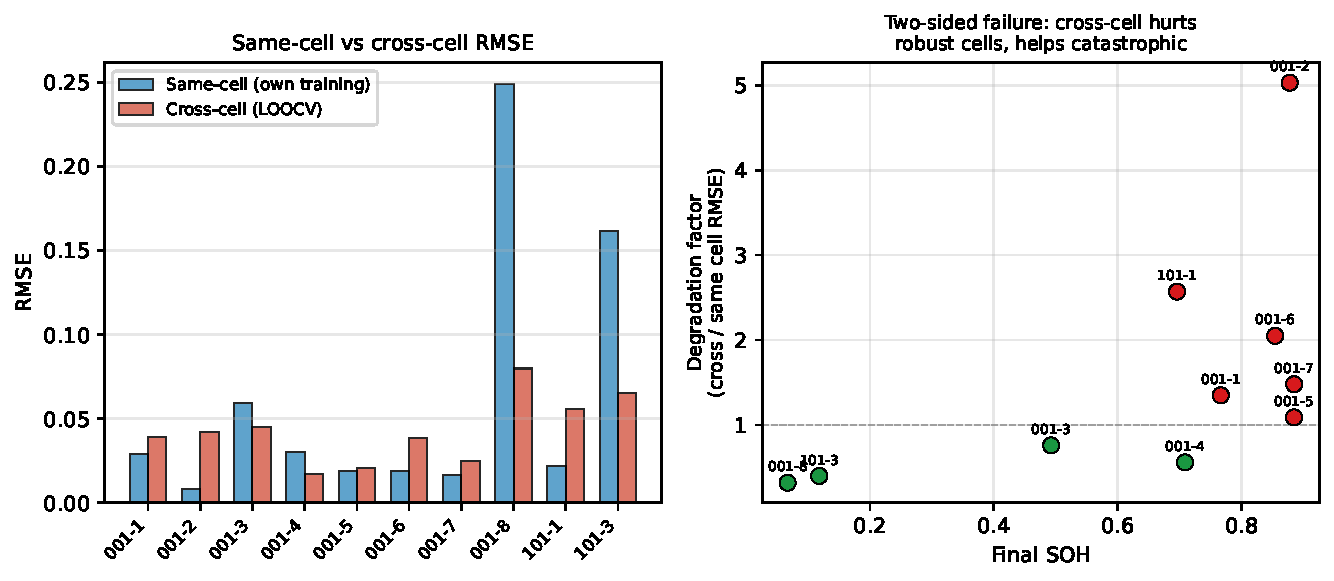
\includegraphics[width=\textwidth]{fig4_loocv}
\caption{G1 LOOCV: same-cell vs cross-cell RMSE at the 50\% split.}
\label{fig:loocv}
\end{figure*}

Leave-one-out cross-validation (LOOCV) on the 10 G1 cells reveals a nuanced
picture (Table~\ref{tab:loocv}, whose factor column gives the
cross-cell/same-cell RMSE ratio, with values below 1 favouring cross-cell).
The pooled cross-cell model (a plain LSTM, $H=64$, $W=20$, trained on the
\emph{full} trajectories of
the other nine cells and tested on the held-out cell) achieves a lower
\textit{mean} RMSE than same-cell training (which uses only the first 50\% of the
held-out cell; 0.049 vs.\ 0.060 at 50\% split), but this average conceals
opposing failure modes:

\begin{table}[htbp]
\caption{Same-cell vs cross-cell RMSE for the 10 G1 cells (50\% split).}
\label{tab:loocv}
\begin{tabular*}{\columnwidth}{@{\extracolsep{\fill}}lrrrr}
\toprule
Cell & SOH$_\text{end}$ & Same-cell & Cross-cell & Factor \\
\midrule
001-1 & 0.767 & 0.0363 & 0.0197 & 0.54$\times$ \\
001-2 & 0.878 & 0.0149 & 0.0262 & 1.77$\times$ \\
001-3 & 0.493 & 0.0938 & 0.0628 & 0.67$\times$ \\
001-4 & 0.709 & 0.0348 & 0.0389 & 1.12$\times$ \\
001-5 & 0.885 & 0.0166 & 0.0340 & 2.04$\times$ \\
001-6 & 0.854 & 0.0153 & 0.0189 & 1.24$\times$ \\
001-7 & 0.885 & 0.0162 & 0.0311 & 1.92$\times$ \\
001-8 & 0.067 & 0.1746 & 0.1183 & 0.68$\times$ \\
101-1 & 0.696 & 0.0424 & 0.0425 & 1.00$\times$ \\
101-3 & 0.118 & 0.1553 & 0.1015 & 0.65$\times$ \\
\midrule
Mean  &       & 0.0600 & 0.0494 & 0.82$\times$ \\
\bottomrule
\end{tabular*}
\end{table}

The cross-cell model is better for 4 of 10 cells, and the largest gains are
on the catastrophic degraders (001-8: same-cell RMSE = 0.175, cross-cell =
0.118; 101-3: 0.155 vs.\ 0.102), where same-cell training on the first 50\%
of a catastrophically failing cell provides a severely biased trajectory
estimate.
But pooling degrades five of the remaining cells by up to 2$\times$ (001-5:
0.017 same-cell vs.\ 0.034 cross-cell; 001-2 and 001-7 are also harmed by
factors of 1.8 to 1.9), and nothing in a cell's early data reveals in advance
whether it will be helped or harmed: the harmed cells are the \emph{most
robust} cells in the population, whose own smooth history is a better guide
than the pooled average.
The split is not sensitive to the training budget: when the cross-cell model
is retrained on only the first 50\% of each source cell (matching the
same-cell information budget), the mean falls to 0.019 vs.\ 0.023 same-cell
and the helped/harmed split remains 6/10, so the two-sided pattern is a
property of pooling itself, not of the data advantage.

Figure~\ref{fig:loocv} makes this pattern visual: the left panel contrasts
same-cell and cross-cell RMSE for each G1 cell, while the right panel plots each
cell's degradation factor against its final SOH, showing cross-cell training
helping the low-SOH catastrophic degraders but hurting the high-SOH robust cells.
This \textbf{two-sided failure mode}, where cross-cell training rescues
catastrophic degraders but unpredictably harms a minority of ordinary cells,
motivates cell-specific adaptation via the fingerprint encoder in
Section~\ref{sec:solution}.

\subsubsection{Early-Life Fingerprint}

The practical value of this insight depends on whether the early SOH
trajectory (observable in the first weeks of deployment) can identify
which cells are likely catastrophic degraders.
Table~\ref{tab:fingerprint} reports Pearson correlations between early-life
statistics and final SOH across 47 MIT LFP cells (SOH$_\text{end}<1$,
excluding 2 capacity-recovery artefacts).

\begin{table}[htbp]
\caption{Correlation of early-life features with final SOH.}
\label{tab:fingerprint}
\begin{tabular*}{\columnwidth}{@{\extracolsep{\fill}}llrrl}
\toprule
$K$ cycles & Feature & $r$ & $p$ & Sig. \\
\midrule
10 & early\_std & $+$0.322 & 0.027 & * \\
10 & max\_drop  & $+$0.371 & 0.010 & * \\
10 & slope      & $-$0.073 & 0.625 &   \\
30 & slope      & $-$0.297 & 0.043 & * \\
50 & slope      & $-$0.380 & 0.008 & ** \\
\bottomrule
\multicolumn{5}{@{}l}{\footnotesize Significance: $^{**}\,p<0.01$; $^{*}\,p<0.05$.}
\end{tabular*}
\end{table}

The 50-cycle slope ($r=-0.38$, $p=0.008$) and 10-cycle max\_drop ($r=+0.37$,
$p=0.010$) are the most predictive individual features
(Figure~\ref{fig:fingerprint}), but with $R^2 \approx 0.14$
these statistics explain only 14\% of the variance in final SOH.
Linear early-life statistics are insufficient for reliable individual-cell
prediction; this motivates the CNN fingerprint encoder, which learns a
nonlinear representation from the full 30-cycle trajectory rather than
hand-crafted summary statistics.

\begin{figure*}[htbp]
\centering
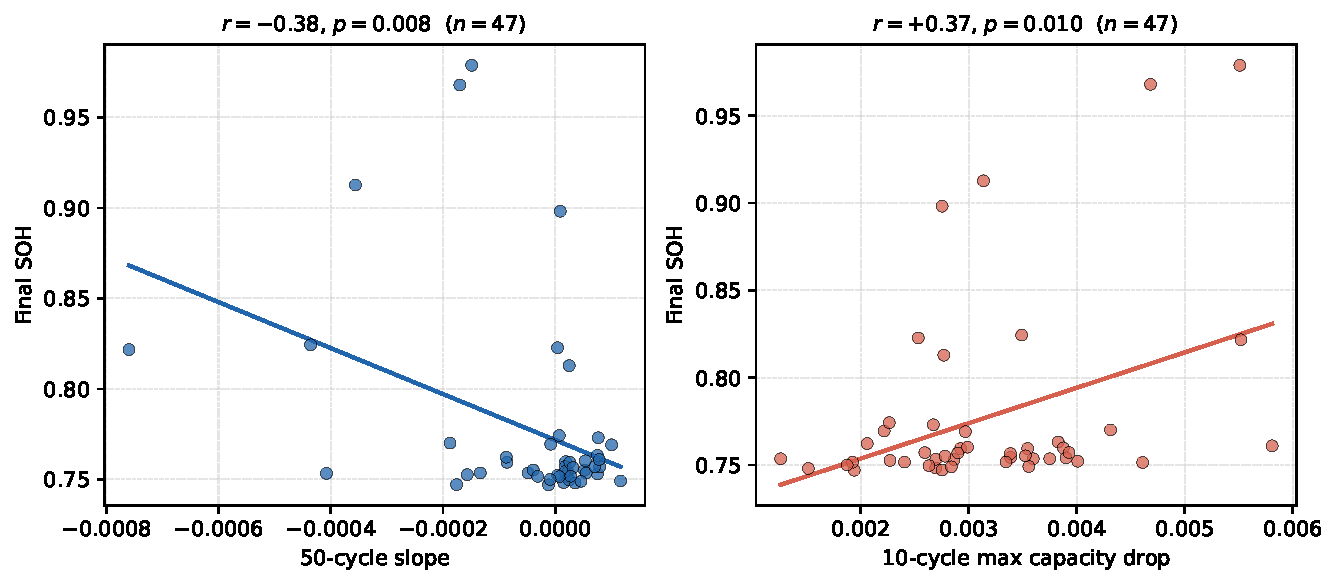
\includegraphics[width=\textwidth]{fig10_fingerprint}
\caption{Early-life predictors of final SOH: 50-cycle slope and 10-cycle maximum capacity drop.}
\label{fig:fingerprint}
\end{figure*}

\subsection{Cross-Condition Transfer Is Dominated by Training-Run
Variance}\label{sec:brittleness}

\begin{table}[htbp]
\caption{Cross-condition transfer RMSE between operating-condition groups.}
\label{tab:brittleness}
\resizebox{\columnwidth}{!}{%
\begin{tabular}{llrr}
\toprule
Train & Test & RMSE & Factor vs G1 LOOCV \\
\midrule
G1 (LOOCV) & G1          & $0.062 \pm 0.065$ & $1.0\times$ (baseline) \\
G1          & G2          & $0.008 \pm 0.002$ & $0.1\times$ \\
G1          & G3          & $0.034 \pm 0.041$ & $0.6\times$ \\
G2          & G3          & $0.145 \pm 0.139$ & $2.4\times$ \\
G1+G2       & G3          & $0.145 \pm 0.133$ & $2.4\times$ \\
\bottomrule
\end{tabular}%
}
\end{table}

Table~\ref{tab:brittleness} reports the cross-condition transfer RMSE
(mean\,$\pm$\,std across the target cells), with the degradation factor giving
each transfer's RMSE relative to the within-distribution G1 LOOCV baseline;
Figure~\ref{fig:brittleness} plots the same values, with the dashed line marking
that baseline.
Two confounds emerge, and together they carry a methodological warning.
First, G1$\rightarrow$G2 (temperature shift only) yields a far lower RMSE
(0.008) than the G1 LOOCV baseline (0.062), not because temperature
transfer is easy, but because G2 cells happen to have smooth, high SOH
trajectories well within the G1 training distribution: cross-condition RMSE
comparisons are confounded by the difficulty distribution of the test set.
Second, and more consequentially, the transfer factors are dominated by
\emph{training-run variance} rather than by the condition shift itself.
Each transfer row is one pooled model, and independent training draws of the
same experiment produce qualitatively different conclusions: an earlier run
of G1$\rightarrow$G3 with library-default (unseeded) initialisation yielded
$2.3\times$ degradation, whereas the deterministic pipeline reported here
yields $0.6\times$, i.e.\ \emph{better} than within-distribution.
Even within Table~\ref{tab:brittleness} the instability is visible:
training on G1 alone transfers to G3 at 0.034, yet \emph{adding} G2 data
(G1+G2$\rightarrow$G3) worsens the same transfer to 0.145, a difference no
condition-shift mechanism explains.
At one-step granularity, cross-condition effects on these data are smaller
than the noise floor of neural-network training itself, another face of the
benchmark saturation established in Section~\ref{sec:baseline}.
We therefore do not claim a cross-condition brittleness effect; the
defensible claims are the test-set difficulty confound and the dominance of
run variance, both of which argue for capability-based evaluation with
uncertainty quantification rather than single-model RMSE comparisons.

The within-distribution baseline used here (G1 LOOCV, $0.062$) trains on the
first 50\% of each source-group cell, identical to the cross-condition
transfers, so every degradation factor in Table~\ref{tab:brittleness} is
computed within one consistent protocol.
It is therefore larger than the full-trajectory cross-cell LOOCV reported in
Section~\ref{sec:variability} ($0.049$), which trains on the complete
trajectories of the other nine cells and so sees their degradation tails; the
two baselines answer different questions and should not be compared directly.

\begin{figure}[htbp]
\centering
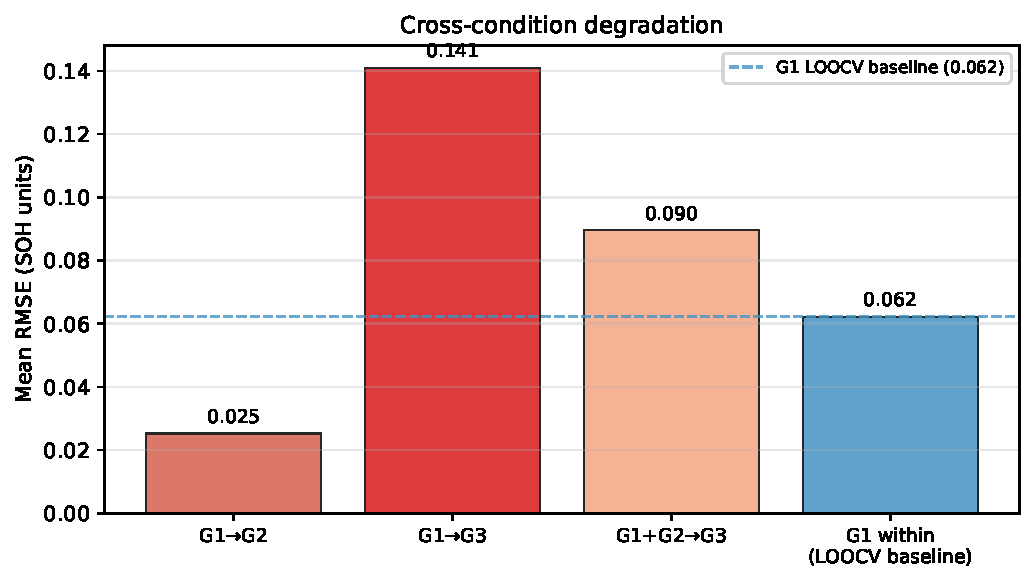
\includegraphics[width=\columnwidth]{fig5_brittleness}
\caption{Mean RMSE for each cross-condition transfer under the deterministic pipeline.}
\label{fig:brittleness}
\end{figure}

\subsection{Requirements for a Robust Predictor}\label{sec:motivation}

The preceding results expose why no single-cell predictor stands out on SIT and
what a better model must instead provide.
The limiting factor is not the sequence model or its hyperparameters but
cell-to-cell variability.
Under nominally identical G1 conditions, per-cell optimised DE-LSTM RMSE still
varies ${\sim}5\times$ across the ten cells
(Section~\ref{sec:baseline}), because a model trained on the early portion of a
single cell's trajectory cannot tell where that cell sits in the manufacturing
distribution: the first half of a catastrophic degrader closely resembles that
of a moderate one.
No amount of per-cell hyperparameter search resolves this, because the missing
information is not present in the individual cell's early history.

Pooling data across cells, the obvious alternative, introduces a two-sided
failure mode (Section~\ref{sec:variability}).
A single model trained on the whole population helps catastrophic degraders,
for which the population average is a better prior than their own ambiguous
early trajectory, but it degrades half of the ordinary cells by up to
2$\times$, and which cells suffer is not predictable a priori.
Neither per-cell tuning nor naive pooling addresses the underlying problem.

These observations, together with the saturation of the one-step metric,
reframe the task.
What matters is not squeezing the last fraction of a percent from a saturated
leaderboard but providing capabilities the leaderboard does not measure: a
degradation prior broad enough to recognise extreme trajectories, prediction
for cells with little or no usable history, and honest uncertainty estimates.
The hybrid model provides the first through pretraining on a large, diverse LFP
corpus (Section~\ref{sec:datasets}), the second through an early-life
fingerprint encoder that enables prediction without target-cell fine-tuning,
and the third through MC-Dropout with conformal calibration.


\section{Proposed Method: Hybrid Model}\label{sec:method}
This section presents the proposed hybrid model: an overview of its three phases,
the architecture and training of each, the mechanism that distinguishes the
fingerprint encoder from conventional fine tuning, and the design of the ablation
used to isolate each component.

\subsection{Framework Overview}\label{sec:framework}

Figure~\ref{fig:methodology} summarises the proposed method in two steps. Step~1
(top) builds the hybrid in three phases: it pretrains on past LFP cells, then, for
each new cell, forms an early-life fingerprint and fine tunes. Step~2 (bottom)
shows the three outputs this supports, one per deployment question (how healthy
the cell is now, which cells will fail, and how long each cell will last), and
pairs each output with the experiment that validates it. Every battery dataset fed
into the model is marked with a battery icon. The core is the three-phase hybrid
that predicts next-cycle SOH, detailed below and evaluated in
Section~\ref{sec:results}.
Phase~1 pretrains the hybrid network, the convolutional fingerprint encoder
together with the LSTM, end-to-end on the chemistry matched MIT dataset to
acquire general LFP degradation knowledge.
Phase~2 applies the pretrained encoder to the first 30 discharge cycles of a
target cell, producing a fingerprint that initialises the LSTM hidden state and
conditions all subsequent predictions.
Phase~3 fine tunes the LSTM on the target cell's training split and performs
MC-Dropout inference to deliver uncertainty-aware predictions whose
prediction intervals are empirically validated rather than merely assumed.

The same early-life representation supports two capabilities developed later in
the paper. An early screen for manufacturing-defective cells reads the discharge
voltage curve rather than the capacity trajectory (Section~\ref{sec:screening}),
and a remaining-useful-life forecaster replaces the one-step head with a direct
multi-horizon decoder (Section~\ref{sec:rul}). The two transfer levers are
distinct: the base hybrid is pretrained on the chemistry-aligned MIT LFP set,
whereas the RUL decoder is pretrained on a 155-cell LFP foundation corpus drawn
from the MIT, HUST, and SNL collections. These two levers are matched to two
different tasks rather than merged into one: one-step SOH is a local prediction
whose accuracy saturates on these smooth large-format trajectories
(Section~\ref{sec:results}), so the chemistry-aligned MIT corpus is sufficient
and additional data brings no measurable gain, whereas remaining-useful-life
forecasting is a long-horizon, data-limited task whose error falls only when the
corpus is enlarged to the full 155-cell collection
(Section~\ref{sec:rul_foundation}). Because that foundation set contains the MIT
cells used for the base hybrid, the two corpora are nested rather than
independent, so the RUL stage extends the SOH stage rather than competing with
it; we keep the two pretraining stages separate only so that each transfer lever
can be isolated in the ablation.

\begin{figure*}[htbp]
\centering
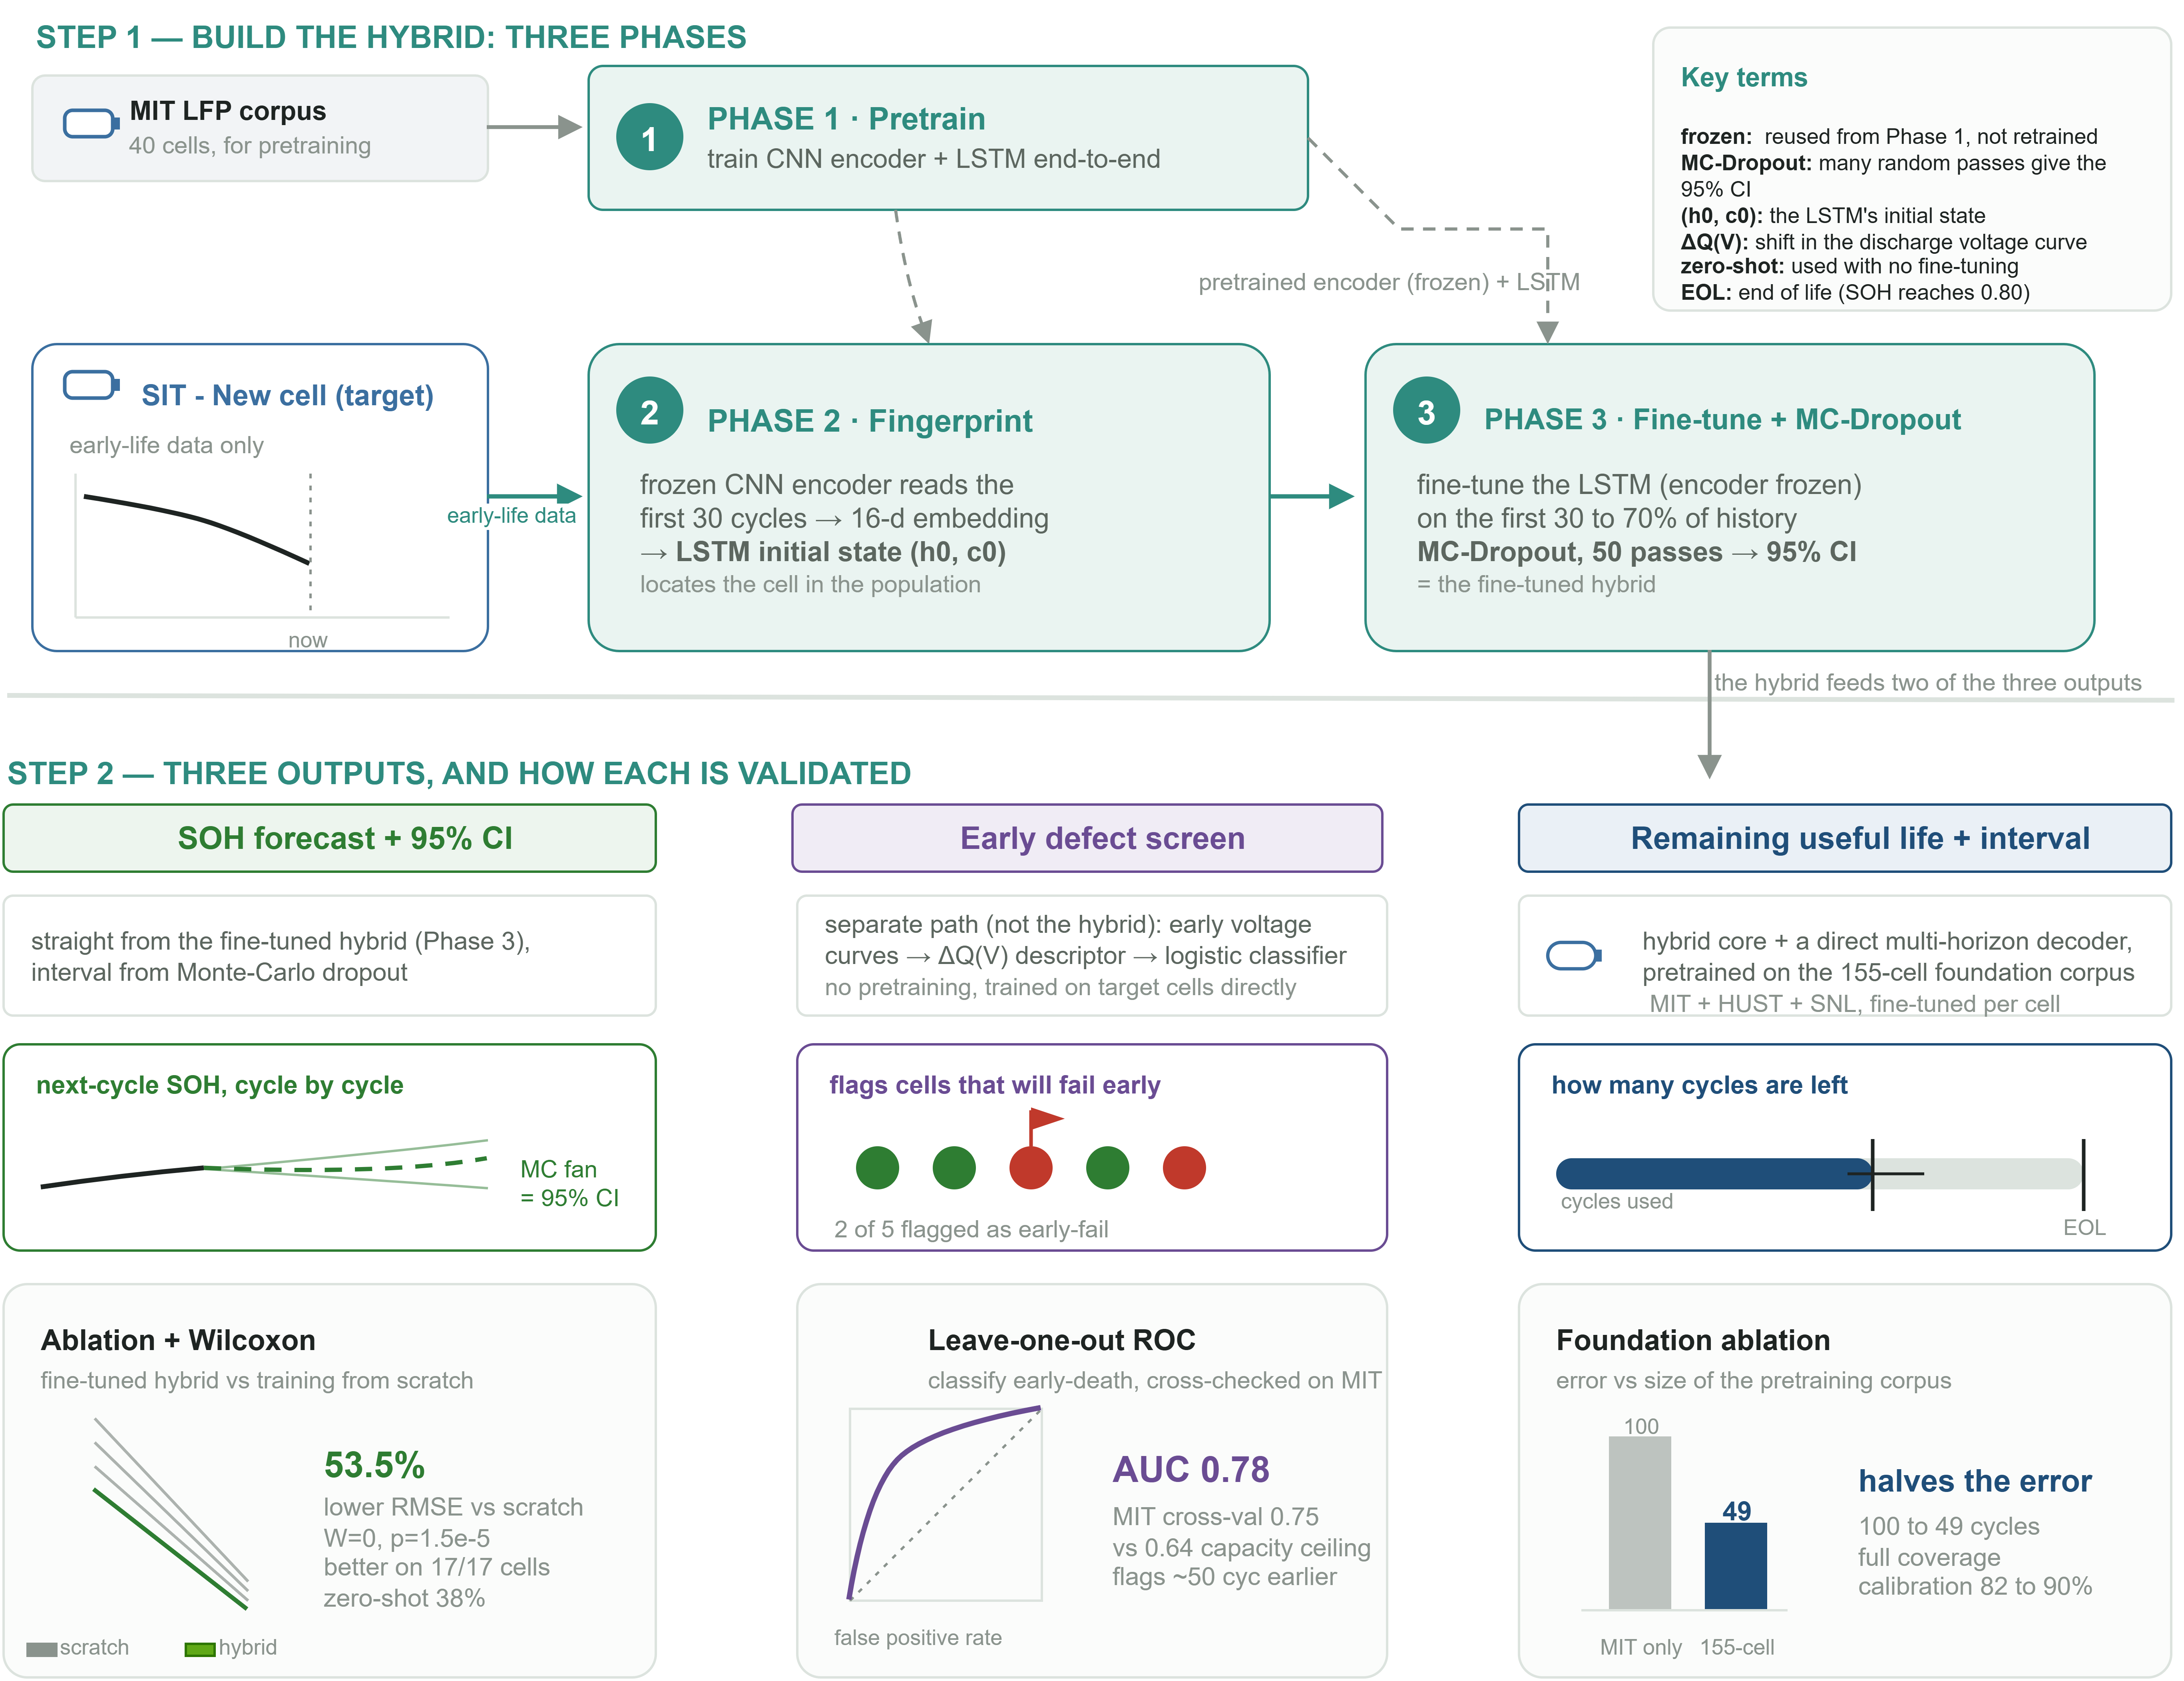
\includegraphics[width=\textwidth]{methodology.png}
\caption{The proposed method: the three-phase hybrid and its three validated outputs.}
\label{fig:methodology}
\end{figure*}

\subsection{Hybrid Model Architecture}\label{sec:hybrid_arch}

The hybrid model operationalises the two capabilities identified in
Section~\ref{sec:motivation} through three phases, drawn as the Step~1 sequence at
the top of Figure~\ref{fig:methodology}:

\subsubsection{Phase 1: MIT Pretraining}
The complete hybrid architecture (the convolutional fingerprint encoder of
Phase~2 together with the LSTM) is pretrained \textit{end-to-end} on the
40-cell MIT LFP corpus (Section~\ref{sec:datasets}).
For each cell, the first 30 cycles form the fingerprint input and the network
is trained to predict every \textit{subsequent} cycle's SOH from a recent
look-back window, minimising next-cycle mean squared error
(LSTM: $H=64$, $W=20$; Adam, learning rate $10^{-3}$; early stopping on a 10\%
validation split).
This single objective jointly learns two things: general LFP degradation
dynamics in the LSTM, and the mapping from early-life trajectory shape to the
LSTM initial state in the fingerprint encoder.
The encoder weights obtained here are reused, and frozen, in Phase~3.

\subsubsection{Phase 2: Convolutional Fingerprint Encoder}
A 1-D convolutional network (two Conv1D layers with 32 and 16 filters
respectively, kernel size 3, followed by global average pooling and a dense
projection) encodes the first 30 SOH cycles of the
target cell into a 16-dimensional embedding vector.
This encoder is the same one trained jointly in Phase~1; its parameters are
not re-learned per target cell.
Two dense layers project this embedding to the LSTM initial hidden state
$h_0$ and cell state $c_0$, conditioning predictions on the individual
cell's observed early behaviour.

Formally, let $\mathbf{s} = [s_1, s_2, \ldots, s_{30}]^{\top} \in \mathbb{R}^{30}$
denote the first 30 normalised discharge capacities of the target cell.
The encoder computes:
\begin{equation}
  \mathbf{z} = \mathrm{GlobalAvgPool}\!\left(
    \mathrm{Conv}_2\!\left(\mathrm{Conv}_1(\mathbf{s})\right)
  \right) \in \mathbb{R}^{16}
  \label{eq:fingerprint}
\end{equation}
\begin{equation}
  h_0 = \tanh(\mathbf{W}_h\,\mathbf{z} + \mathbf{b}_h), \qquad
  c_0 = \tanh(\mathbf{W}_c\,\mathbf{z} + \mathbf{b}_c)
  \label{eq:h0c0}
\end{equation}
where $\mathbf{z}$ is the fingerprint embedding from Equation~\eqref{eq:fingerprint},
$\mathbf{W}_h$ and $\mathbf{W}_c$ are the weight matrices of the two dense
projection layers, $\mathbf{b}_h$ and $\mathbf{b}_c$ are their bias vectors, and
$h_0$ and $c_0$ are the resulting LSTM initial hidden and cell states.
The critical point is that $\mathbf{s}$ is treated as a \textit{static shape},
not a sequence to continue: the CNN pools over all 30 cycles simultaneously to
extract curvature, rate of decline, and early-knee features that characterise
where this cell sits in the manufacturing distribution relative to the
pretrained population.

\subsubsection{Phase 3: Fine tuning and MC-Dropout}
The pretrained LSTM is fine tuned
on the first \textit{train\_pct}\% of the target cell's SOH trajectory,
starting from the cell-specific initial state $(h_0, c_0)$ produced by the
fingerprint encoder.
The fingerprint encoder weights, learned in Phase~1, are held \textit{frozen}
throughout fine tuning; only the LSTM and output-layer weights are updated.
Training and inference use fixed-length look-back windows of $W=20$ cycles drawn
from the target cell's SOH. Each window is processed independently: the LSTM is
re-initialised to the fingerprint-derived state $(h_0, c_0)$ at the first step of
every window rather than carrying hidden state across windows, so each prediction
is conditioned on both the cell-level fingerprint and its local $W$-cycle history.
The fine tuning objective is:
\begin{equation}
  \mathcal{L}_{\mathrm{FT}} = \frac{1}{K}\sum_{t=1}^{K}\!\left(\hat{y}_t - y_t\right)^2,
  \quad K = \left\lfloor \frac{p}{100} \cdot T \right\rfloor
  \label{eq:ft_loss}
\end{equation}
where $y_t$ is the observed SOH at cycle $t$, $\hat{y}_t$ is the model
prediction, $T$ is the total cycle count of the target cell, and $p \in
\{30, 50, 70\}$.
Dropout (rate 0.2) applied to the LSTM output during both training and
inference provides uncertainty estimates via 50 stochastic forward passes.
The 95\% prediction interval is $\hat{y} \pm 1.96\,\hat{\sigma}$ (an approximate
MC-Dropout interval, not a calibrated confidence interval), where $\hat{\sigma}$
is the empirical standard deviation across the 50 passes.

\subsection{Pretraining-Run Variance and Checkpoint Selection}\label{sec:selection}

Pretraining a neural network is stochastic: independent runs on the identical
corpus, differing only in random initialisation, converge to representations of
very different transfer quality.
Across five deterministic pretraining runs of Phase~1, downstream SIT
improvement over scratch ranged from $-32\%$ to $+52\%$: three runs learned
genuine degradation dynamics while two collapsed toward a persistence
solution that transfers poorly.
Crucially, \emph{source-domain criteria failed to identify the collapsed
runs}: MIT validation loss was essentially identical for good and collapsed
runs (${\approx}3.4\times10^{-3}$), one-step-ahead RMSE on held-out MIT cells
was \emph{inverted} (collapsed runs win it, because persistence excels at
one-step prediction), and recursive multi-step rollout was uninformative.

We therefore adopt a simple target-domain selection protocol:
\begin{enumerate}
  \item pretrain $k=5$ candidate checkpoints with independent seeds;
  \item evaluate each candidate's fine-tuned RMSE on the three designated
        \emph{calibration cells} (Section~\ref{sec:eval});
  \item deploy the checkpoint with the lowest mean calibration RMSE.
\end{enumerate}
The calibration cells are chosen by an a-priori rule (the numerically first
cell of each condition group) and are excluded from all reported results.
The protocol is robust to the choice of calibration cells: exhaustively
enumerating all $\binom{20}{3}=1140$ possible three-cell calibration sets,
95.5\% select a checkpoint with positive test improvement.
In deployment terms the protocol is realistic: a manufacturer qualifying a
battery product retains laboratory cells of that product, and three such
cells suffice.
All results in Section~\ref{sec:results} use the selected checkpoint; the
full five-run sensitivity study is released with the code.

\subsection{Mechanism Contrast: Fingerprint Encoder vs.\ Fine Tuning}\label{sec:mechanism}

Although Phases 2 and 3 both draw on the same early-cycle SOH data, they
use it in fundamentally different ways, a distinction that directly motivates
the ablation study in Section~\ref{sec:ablation_design}.
Table~\ref{tab:mechanism_contrast} makes this contrast explicit.

\begin{table*}[!t]
\caption{Comparison of the two mechanisms that use early-cycle SOH data.}
\label{tab:mechanism_contrast}
\centering
\begin{tabularx}{\textwidth}{l X X}
\toprule
 & \textbf{Incremental fine tuning} & \textbf{Fingerprint encoder} \\
\midrule
\textit{Input view} & Time series $s_1 \to s_2 \to \cdots \to s_K$ & Static shape $\mathbf{s} \in \mathbb{R}^{30}$ \\
\textit{Operation}  & Adjust LSTM weights $\theta$ to minimise $\mathcal{L}_{\mathrm{FT}}$ & Map shape to $(h_0, c_0)$ via CNN \\
\textit{Output}     & Updated model weights & Cell-specific initial state \\
\textit{Question answered} & What comes next in this sequence? & What type of degrader is this cell? \\
\textit{Limitation} & Ambiguous for extreme cells in the first $p$\% & Requires a diverse pretraining corpus \\
\bottomrule
\end{tabularx}
\end{table*}

For cells at the extremes of the manufacturing distribution
(catastrophically fast: cell 001-8; exceptionally robust: cells 001-5
and 001-7), the first 50\% of the SOH trajectory is \textit{ambiguous}:
it resembles a moderate degrader.
Fine tuning on this ambiguous first half fits a moderate trajectory and
projects it forward, substantially underestimating the second half.
The fingerprint encoder, by contrast, conditions the LSTM on the early-life
trajectory shape (curvature and rate of decline across the first 30 cycles),
placing the prediction in the context of the pretrained population.
Whether this conditioning encodes precise cell \emph{identity} or a more
generic in-distribution prior is an empirical question; a shuffled-fingerprint
control in Section~\ref{sec:results} shows the latter dominates, and we
interpret the mechanism accordingly.

\subsection{Ablation Study Design}\label{sec:ablation_design}

To isolate the contribution of each hybrid component, four configurations
are compared:
\begin{enumerate}
  \item \textbf{Scratch LSTM}: Train the hybrid's LSTM backbone
        ($H{=}64$, $W{=}20$) from scratch on the target cell's training split
        only, with no pretraining, no fingerprint, and no differential-evolution
        hyperparameter search. This is the ablation control for the hybrid and is
        distinct from the DE-optimised DE-LSTM baseline of
        Section~\ref{sec:baseline}; the two therefore differ in RMSE.
  \item \textbf{Zero-shot (pretrain + fingerprint, no fine tuning)}: the MIT
        pretrained model with the fingerprint-derived initial state applied
        directly to the target cell, with \textit{no fine tuning} on target
        data (here \textit{zero-shot} denotes the absence of target-cell fine
        tuning; the first 30 cycles are still used to compute the fingerprint).
        Isolates the value of pretraining and the fingerprint before any
        target-cell adaptation.
  \item \textbf{Pretrain + fine tune (no fingerprint)}: MIT pretrained
        model fine tuned on the target cell's training split, but without
        the fingerprint encoder.
        Quantifies the marginal value of the fingerprint over fine tuning alone.
  \item \textbf{Full hybrid}: All three phases (pretrain + fingerprint + fine-tune).
\end{enumerate}

\subsection{Reproducibility and Determinism}\label{sec:repro}

All experiments run under a fully deterministic configuration: a single
global seed set via \texttt{tf.keras.utils.set\_random\_seed} (which, unlike
\texttt{tf.random.set\_seed} alone, also seeds Keras weight initialisers),
TensorFlow op-determinism enabled, and float32 precision throughout.
Under this configuration every number reported in this paper reproduces
byte-for-byte from a fresh clone of the released code.
The repository includes a single-command verification script
(\texttt{verify\_determinism.sh}) that exercises each experiment family's
actual training and inference code path twice in separate processes and
byte-compares the outputs, so that reviewers and users can confirm
determinism on their own hardware before relying on the pipeline.
We adopted this discipline after observing that library-default (unseeded)
training produced run-to-run variation large enough to alter experimental
conclusions (Sections~\ref{sec:baseline} and~\ref{sec:brittleness}); we
regard it as a necessary condition for benchmark claims in this field.


\section{Hybrid Model Evaluation}\label{sec:results}
This section evaluates the hybrid through an ablation isolating each component,
the main accuracy results on the 17 SIT test cells, conformal calibration of its
uncertainty intervals, and a cross-dataset validation of the chemistry alignment
principle.

\subsection{Ablation Study and Main Results}\label{sec:solution}

We first isolate the contribution of each component, then report the full
hybrid's accuracy and calibration across the 17 test cells (the three calibration cells of Section~\ref{sec:eval} are excluded from every reported metric).

\subsubsection{Ablation Study}

\begin{table}[htbp]
\caption{Ablation study: contribution of each hybrid component (50\% split).}
\label{tab:ablation}
\resizebox{\columnwidth}{!}{%
\begin{tabular}{lrrr}
\toprule
Configuration & RMSE & Improvement vs scratch & PI Coverage \\
\midrule
Scratch LSTM             & $0.043 \pm 0.050$ & (baseline)  & n/a   \\
Zero-shot (MIT + FP, no FT) & $0.025 \pm 0.026$ & 38.2\%$^\ddag$   & 77.3\%\\
Pretrain + FT (no fing.) & $0.017 \pm 0.016$ & 47.7\%$^\ddag$   & 79.8\%\\
Full hybrid (proposed)   & $\mathbf{0.014 \pm 0.013}$ & \textbf{53.5\%}$^\ddag$  & 82.1\%\\
\bottomrule
\multicolumn{4}{l}{$^\ddag$ Wilcoxon $p<0.001$ vs scratch.}
\end{tabular}%
}
\end{table}

\begin{figure}[htbp]
\centering
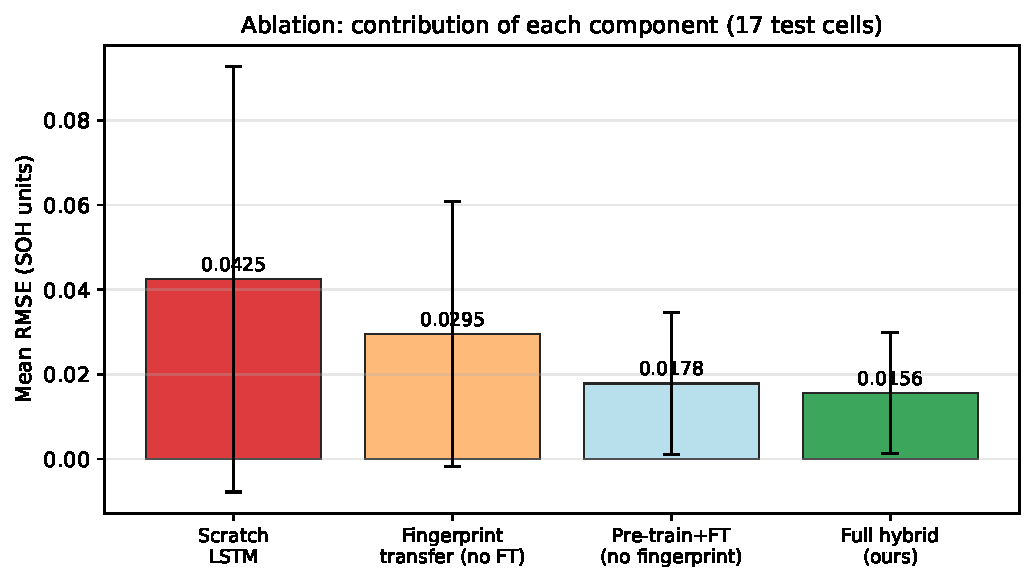
\includegraphics[width=\columnwidth]{fig6_ablation}
\caption{Ablation study: mean RMSE per configuration (50\% split).}
\label{fig:ablation}
\end{figure}

Table~\ref{tab:ablation} and Figure~\ref{fig:ablation}, which plots the same
mean RMSE per configuration, show that every component contributes and the
effects compose monotonically: zero-shot transfer (pretrained model with the
fingerprint-derived initial state, \emph{no} fine tuning on target data)
already achieves a 38.2\% improvement over scratch and beats scratch on all
17 test cells; adding fine tuning without the fingerprint reaches 47.7\%;
and the full hybrid reaches 53.5\% (all Wilcoxon $p<0.001$).
Three observations stand out.
First, the zero-shot configuration is the capability no other evaluated
method offers: RMSE 0.025 for a cell with \emph{no} target-cell training,
from 30 observed cycles, recovering roughly 70\% of the full hybrid's
benefit before any adaptation is possible.
Second, the fingerprint and fine tuning are complementary rather than
redundant: the fingerprint on top of pretraining+fine tuning still reduces
RMSE from 0.017 to 0.014.
Third, a shuffled-fingerprint control clarifies the mechanism: replacing each
test cell's fingerprint with another cell's raises full-hybrid RMSE only from
0.0141 to 0.0146.
The conditioning therefore works chiefly by placing the LSTM in the
\emph{pretrained population's} operating regime (any in-distribution
early-life shape suffices) rather than by encoding a precise cell identity,
which is consistent with the two mechanisms remaining complementary
(Section~\ref{sec:mechanism}).
Prediction-interval coverage improves in the same monotone order
(77.3\%~$\rightarrow$~79.8\%~$\rightarrow$~82.1\%), so with a
well-selected pretrained checkpoint there is no accuracy versus calibration
trade-off among the configurations.

\subsubsection{Hybrid Accuracy Across Operating Conditions}

\begin{table}[htbp]
\caption{Full hybrid results by operating-condition group (50\% split).}
\label{tab:hybrid_main}
\resizebox{\columnwidth}{!}{%
\begin{tabular}{lrrrrr}
\toprule
Group & $n$ & Hybrid RMSE & Scratch RMSE & Improvement & PI Coverage \\
\midrule
G1 (25\,\textcelsius, 1C) & 9 & $0.015\pm0.012$ & $0.035\pm0.034$ & 44.0\% & 80.3\% \\
G2 (40\,\textcelsius, 1C) &  3 & $0.005\pm0.002$ & $0.016\pm0.013$ & 56.8\% & 79.0\% \\
G3 (40\,\textcelsius, 2C) &  5 & $0.019\pm0.016$ & $0.073\pm0.077$ & 68.8\% & 87.1\% \\
\midrule
All SIT (test)            & 17 & $0.014\pm0.013$ & $0.043\pm0.050$ & 53.5\% & 82.1\% \\
\bottomrule
\end{tabular}%
}
\end{table}

The full hybrid model achieves a statistically significant improvement over
scratch LSTM across the 17 test cells (Wilcoxon $W=0$, $p=1.5\times10^{-5}$;
hybrid better in 17/17 cells).
Table~\ref{tab:hybrid_main} breaks the hybrid and scratch RMSE, the mean
improvement, and the PI coverage down by operating-condition group.
Figure~\ref{fig:hybrid_percell} shows the per-cell results: the top panel
compares each cell's scratch and hybrid RMSE, while the bottom panel gives the
corresponding per-cell improvement of the hybrid over scratch (positive for
every test cell; the smallest improvement is 14.9\% on cell 101-1).

On the one-step metric itself, every method is bunched on a saturated scale:
the hybrid's mean RMSE is 0.0212, 0.0141 and 0.0156 at the 30\%, 50\% and 70\%
splits (Figure~\ref{fig:method_comparison}), the per-cell-tuned DE-LSTM reaches
0.0118 and 0.0105 at 50\% and 70\%, and even a trivial linear autoregressor sits
near 0.005, differences that carry little information on this saturated benchmark
(Section~\ref{sec:baseline}). The hybrid's decisive advantage is therefore not a
marginal one-step number but a set of capabilities that no other method on the
leaderboard provides. It is the only method that operates with no target training
at all (zero-shot, 0.025), the only method that quantifies uncertainty
(Section~\ref{sec:conformal}), and the only one validated across three
manufacturers (MIT, SIT and LISHEN), two chemistries (LFP and LCO) and three
operating conditions (Section~\ref{sec:cross_dataset}), whereas PA-LSTM, GA-LSTM
and DE-LSTM provide point estimates only, for cells that already have an
established history. On the cells that matter most for deployment, the
catastrophic degraders, this advantage is also an accuracy advantage, as the
next paragraph shows.

Within G1, the hybrid is particularly effective for catastrophic degraders
(Figure~\ref{fig:prediction}):
cell 001-8 (SOH$_\text{end}=0.067$) improves 58.2\%
(0.041 vs.\ 0.098 scratch); cell 101-3 (SOH$_\text{end}=0.118$) improves
81.1\% (0.016 vs.\ 0.083).
Both gains are driven by the MIT pretraining, which has encountered
comparable extreme-degradation trajectories in the training population,
a trajectory the scratch model cannot learn from 50\% of a single
catastrophic cell's history.
Figure~\ref{fig:prediction} plots the hybrid's predicted versus actual SOH with
95\% MC-Dropout uncertainty bands on the held-out second half (50\% split) for
three representative cells, a robust G1 cell, the catastrophic degrader 001-8,
and a condition-shifted G3 cell, with the training portion shaded and the
train/test boundary dashed.
Across all three the hybrid tracks both gentle and catastrophic trajectories, and
the prediction interval widens where degradation is steepest.

For G3 test cells (40\,\textcelsius/2C), the hybrid achieves mean RMSE of
0.019, a 68.8\% improvement over the scratch LSTM given the same 50\% G3 fine
tuning data (0.073; Table~\ref{tab:hybrid_main}), by combining MIT-learned
generic LFP priors with that fine tuning.
Cold cross-condition transfer (a G1-trained model applied to G3 with no G3
data) is not a stable reference point, since Section~\ref{sec:brittleness}
showed such estimates are dominated by training-run variance; the comparison
against the equally-fine-tuned scratch model above is the fair like-for-like
measure of the hybrid's contribution.
The G3 conclusions are not an artefact of cell 003-5 (the SOH$>$1
capacity-recovery cell): excluding it, the four remaining G3 test cells give a
hybrid RMSE of 0.014 (scratch 0.039), a 65.7\% mean per-cell improvement versus
68.8\% with 003-5 included, so the artefact slightly inflates but does not
drive the result.

\begin{figure*}[htbp]
\centering
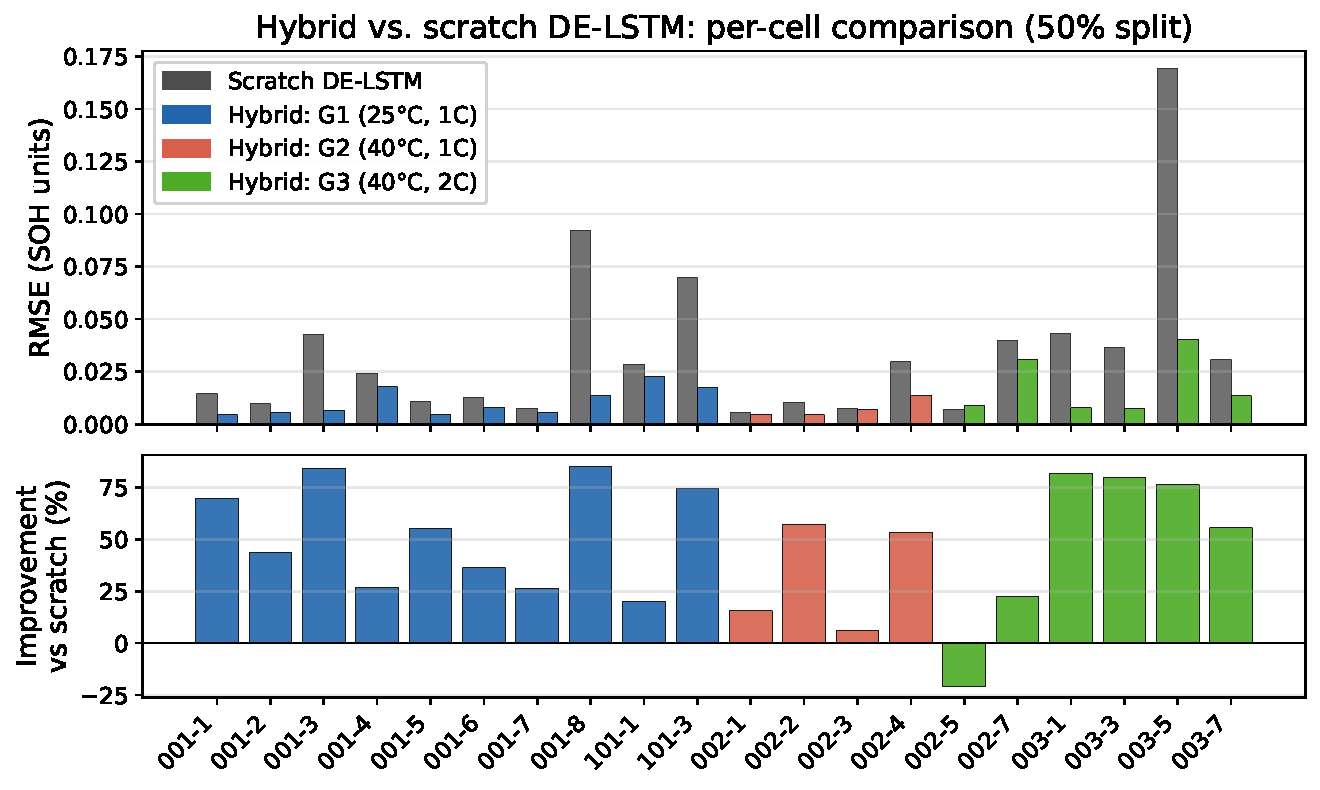
\includegraphics[width=\textwidth]{fig7_hybrid}
\caption{Hybrid vs.\ scratch LSTM on the SIT cells (50\% split).}
\label{fig:hybrid_percell}
\end{figure*}

\begin{figure*}[htbp]
\centering
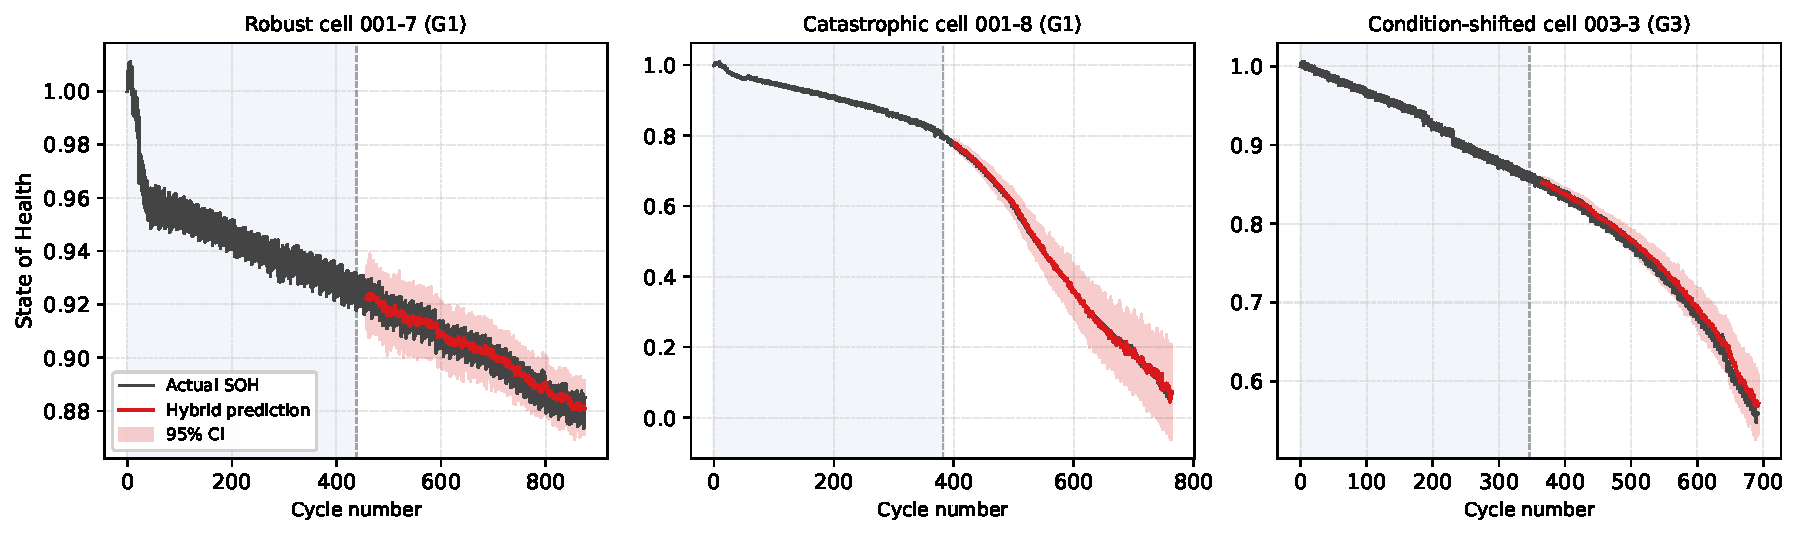
\includegraphics[width=\textwidth]{fig11_prediction}
\caption{Hybrid predicted versus actual SOH with 95\% MC-Dropout uncertainty bands (50\% split).}
\label{fig:prediction}
\end{figure*}

\subsubsection{Conformal Calibration of the Uncertainty
Intervals}\label{sec:conformal}

The raw MC-Dropout intervals are approximate (Section~\ref{sec:hybrid_arch})
and under-cover in practice: pooled over the 17 test cells, the empirical
coverage of nominal 50/80/90/95/99\% intervals is 41/68/78/84/91\%
(Figure~\ref{fig:calibration}, left).
We correct this with split-conformal prediction~\cite{angelopoulos2021gentle}
using the three calibration cells already reserved for checkpoint selection:
the normalised scores $|y_t-\hat{y}_t|/\hat{\sigma}_t$ are collected on the
calibration cells, their 95th percentile $q_{95}$ replaces the Gaussian 1.96,
and test-cell intervals become $\hat{y}_t \pm q_{95}\,\hat{\sigma}_t$.
This raises 95\% coverage from 84.4\% to \textbf{93.9\%} on the test cells
with no target-cell labels beyond the calibration set
(Figure~\ref{fig:calibration}, right).
Coverage reaches at least 92\% on 15 of 17 cells; the two exceptions are the
catastrophic degrader 001-8 (67\%) and the recovery artefact 003-5 (56\%),
whose error distributions differ structurally from anything in the
calibration set, a reminder that conformal guarantees assume
exchangeability, which extreme manufacturing outliers violate.
The full hybrid is the only method in Table~\ref{tab:method_comparison} that
produces uncertainty intervals at all; with conformal correction those
intervals become trustworthy enough for BMS threshold logic on typical cells,
while flagged outliers still require conservative handling.

\begin{figure}[htbp]
\centering
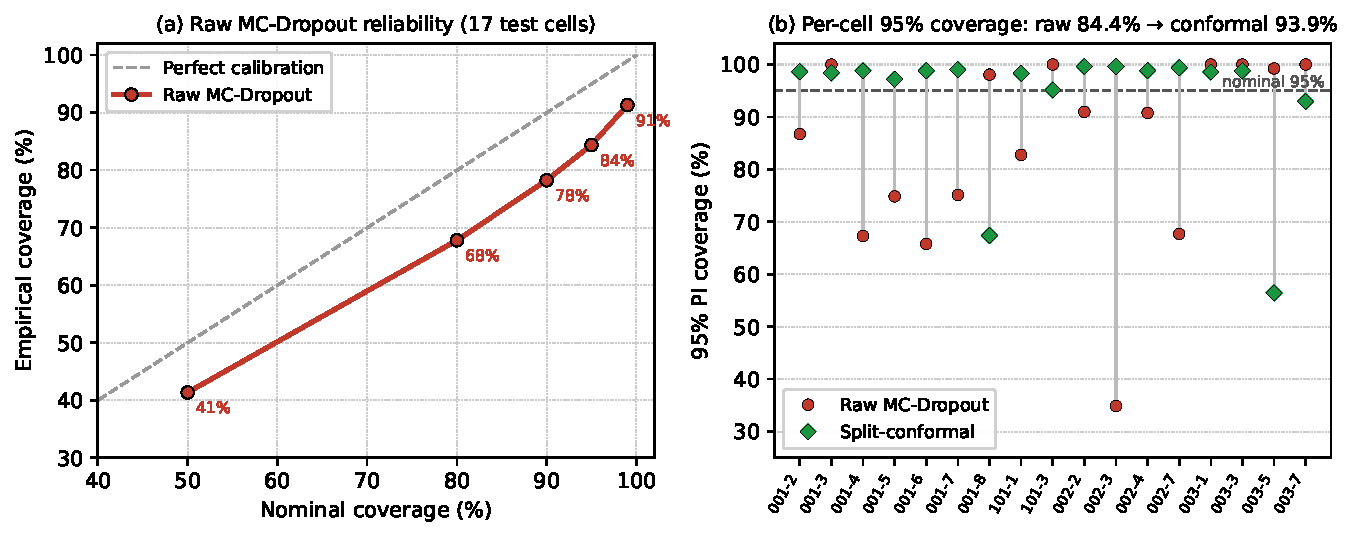
\includegraphics[width=\columnwidth]{fig13_calibration}
\caption{Uncertainty calibration on the 17 test cells.}
\label{fig:calibration}
\end{figure}

\subsubsection{Uncertainty Calibration: The Chemistry Alignment Principle}

\begin{figure*}[htbp]
\centering
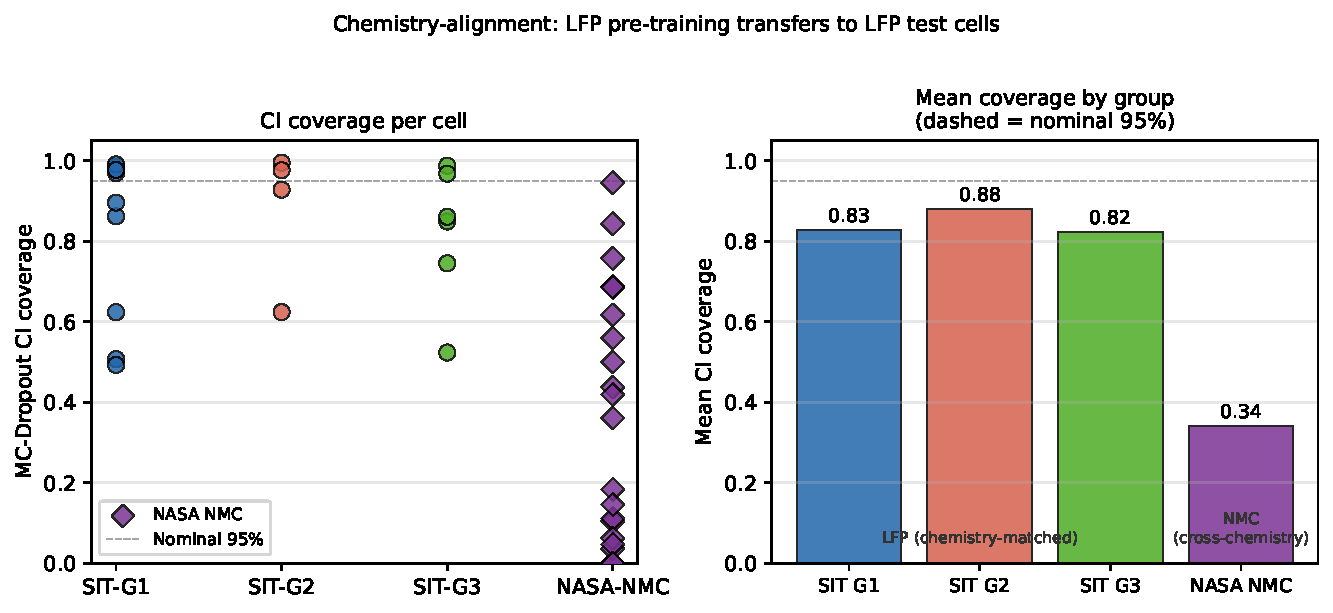
\includegraphics[width=\textwidth]{fig8_coverage}
\caption{MC-Dropout 95\% PI empirical coverage by dataset and group.}
\label{fig:coverage}
\end{figure*}

Figure~\ref{fig:coverage} plots the empirical 95\% PI coverage per cell (left)
and averaged per dataset group (right), and reveals a striking pattern: PI
coverage on SIT LFP cells (82.1\% mean) is nearly double that on NASA LCO
cells (43.1\%), despite using the same MC-Dropout rate (0.2) and the same
nominal 95\% target.
The most prominent structural difference is chemistry: the MIT pretraining data
are LFP cells (matched to SIT), whereas NASA cells are LCO (LiCoO$_2$~\cite{saha2007battery}; mismatched). The
datasets also differ in cell format, laboratory and cycling protocol, so
chemistry is the most likely, but not the only possible, contributor to the
coverage gap; the cross-dataset study below helps disentangle it.

This \textbf{chemistry alignment principle} has a practical implication for
BMS deployment: transfer learning preserves uncertainty calibration only
when the pretraining and deployment chemistries are matched.
Deploying a model pretrained on LFP data to LCO cells not only degrades
point estimate accuracy but also destroys uncertainty calibration, producing
overconfident predictions that could mask true risk.
Post-hoc calibration (conformal prediction~\cite{angelopoulos2021gentle}
or isotonic regression) is required when chemistry is mismatched.

\subsection{Cross-Dataset Validation of the Chemistry Alignment
  Principle}\label{sec:cross_dataset}

The analysis in Section~\ref{sec:solution} established the chemistry alignment
principle from a single source-target pair (MIT$\rightarrow$SIT).
To verify that this finding generalises, we evaluate the hybrid framework
across ten pairwise transfer scenarios spanning three LFP datasets
(MIT Severson~\cite{severson2019data}, SIT, and LISHEN 40\,Ah LFP) and one
LCO dataset (NASA 18650).
The LISHEN dataset~\cite{lishen_zenodo} provides three industrial-scale LFP
cells (40\,Ah) cycled at 2C with 20\% depth of discharge (DOD) regular cycles and full-discharge
reference tests every tenth cycle, offering a third independent LFP
pretraining source distinct from both MIT and SIT in cell format, capacity,
and cycling protocol.

\begin{table*}[htbp]
\centering
\caption{Cross-dataset transfer matrix: RMSE improvement over scratch LSTM.}
\label{tab:cross_dataset}
\begin{tabular*}{\textwidth}{@{\extracolsep{\fill}}clllrrr}
\toprule
Sc. & Source & Target & Chem. & ZS+FP & PT+FT & Hybrid \\
\midrule
\multicolumn{7}{@{}l}{\textit{LFP$\leftrightarrow$LFP (chemistry matched)}} \\
A & MIT (40\,cells) & SIT        & LFP & $+$38.2\% & $+$47.7\% & $+$53.5\% \\
G & MIT (40\,cells) & LISHEN     & LFP & $+$80.2\% & $+$66.2\% & $+$64.5\% \\
B & SIT (20\,cells) & MIT        & LFP & $+$19.6\% & $+$57.1\% & $+$59.5\% \\
H & SIT (20\,cells) & LISHEN     & LFP & $-$22.6\% & $+$46.1\% & $+$38.6\% \\
N & LISHEN (3\,cells) & MIT      & LFP & $+$14.6\% & $+$4.7\% & $+$4.1\% \\
M & LISHEN (3\,cells) & SIT      & LFP & $-$24.6\% &  $+$5.8\% &  $+$5.2\% \\
\midrule
\multicolumn{7}{@{}l}{\textit{LCO$\leftrightarrow$LFP (chemistry-mismatched)}} \\
C & MIT (LFP) & NASA (LCO) & cross & $+$15.6\% & $+$8.8\% & $+$8.9\% \\
D & SIT (LFP) & NASA (LCO) & cross & $+$4.8\% & $+$21.6\% & $+$21.6\% \\
E & NASA (LCO) & SIT (LFP) & cross & $+$26.8\% & $+$44.1\% & $+$43.1\% \\
F & NASA (LCO) & MIT (LFP) & cross & $+$37.2\% & $+$59.8\% & $+$59.5\% \\
\bottomrule
\end{tabular*}
\end{table*}

\begin{figure*}[htbp]
\centering
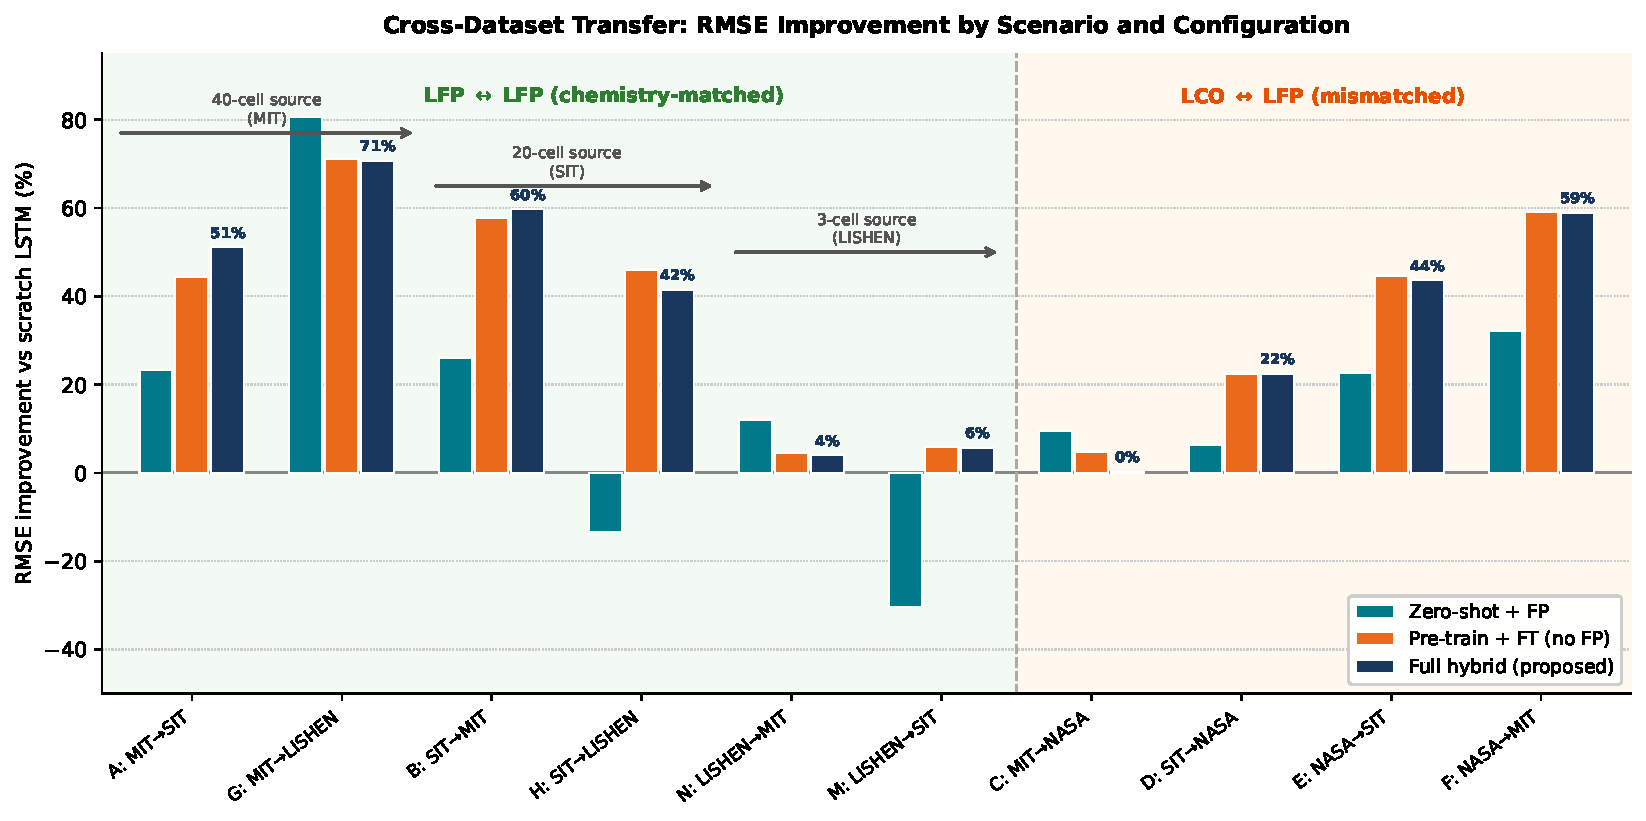
\includegraphics[width=\textwidth]{fig9_cross_dataset}
\caption{Cross-dataset RMSE improvement over scratch LSTM across all ten
transfer scenarios.}
\label{fig:cross_dataset}
\end{figure*}

Scenario~A (MIT$\rightarrow$SIT) repeats the main ablation of
Table~\ref{tab:ablation}, included here for reference.
In Table~\ref{tab:cross_dataset}, the ten scenarios are grouped by chemistry
alignment (LFP$\leftrightarrow$LFP matched, LCO$\leftrightarrow$LFP mismatched)
and negative values denote degradation relative to scratch.
Together with Figure~\ref{fig:cross_dataset}, the results support three findings.

\subsubsection{Fine tuning is the dependable adaptation mechanism}
Pretraining plus fine tuning improves over scratch in \emph{all ten}
scenarios ($+$4.7\% to $+$66.2\%, mean 36.2\%), and the full hybrid tracks
it closely (mean 35.9\%), being best or within one point of best in six of
ten (A, B, D, E, F and~M).
Whatever the source corpus, chemistry, or cell format, fine tuning a
pretrained model on the target cell's history is never worse than training
from scratch in these experiments, which makes it the mechanism a
practitioner can rely on when facing an unfamiliar dataset pair.
The weakest transfers (M and~N, both below 6\%) share one cause: the 3-cell
LISHEN corpus is too narrow a pretraining source for either mechanism.

\subsubsection{Zero-shot conditioning is a distinct capability, not a
universal accuracy win}
Zero-shot performance varies far more across scenarios ($-$24.6\% to
$+$80.2\%) than fine tuning does.
It is strongly positive precisely where the pretrained population resembles
the deployment population: the paper's primary scenario~A
(MIT$\rightarrow$SIT, $+$38.2\%) and scenario~G (MIT$\rightarrow$LISHEN,
$+$80.2\%), both large LFP corpora transferring to LFP targets.
It fails when the source poorly spans the target (H and M, both negative:
SIT's 20 heterogeneous cells and LISHEN's 3 cells do not cover each other's
regimes), because the fingerprint places a cell within the
\emph{pretraining} population's degradation distribution, and that placement
misleads when the distribution does not contain the target's behaviour.
The correct reading is therefore about regime, not rank: zero-shot
conditioning is the only option during the first weeks of deployment, before
any fine-tuning history exists, and it is trustworthy exactly when the
practitioner can match pretraining chemistry and corpus breadth to the
deployment population, precisely the condition a battery manufacturer
qualifying one product line can guarantee.

\subsubsection{Chemistry mismatch reduces accuracy gains and destroys
calibration}
Across the four cross-chemistry scenarios (C to F), hybrid improvement ranges
from 8.9\% to 59.5\% (mean 33.3\%), against 38.6\% to 64.5\% (mean
54.0\%) for the adequately resourced matched-LFP scenarios (A, B, G, H).
The sharper signal is calibration: the PI coverage analysis from
Section~\ref{sec:solution} (82\% LFP$\rightarrow$LFP vs 43\%
LFP$\rightarrow$LCO) shows that the RMSE improvement metric understates the
damage from chemistry mismatch.
The model can remain reasonably accurate in point estimates while becoming
severely overconfident in its uncertainty intervals, the failure mode most
dangerous for BMS deployment, and one invisible to every uncertainty-free
method in Table~\ref{tab:method_comparison}.


\section{Early Detection of Manufacturing-Defective Cells}\label{sec:screening}
% Early detection of manufacturing-defective cells. Style: no em or en dashes; short captions.
Section~\ref{sec:problem} established that cell-to-cell variability dominates within the G1
group, where nominally identical cells span a thirteenfold range in final SOH. A practical
question follows. Can the defective cells be identified early, before their capacity has visibly
diverged? We find that they can, but only from the shape of the discharge voltage curve, not from
any scalar health indicator.

\subsection{Scalar indicators are blind within a group}\label{sec:screen_scalar}
Within G1, the early-life value and slope of the discharge capacity, the surface-temperature
resistance proxy, the coulombic efficiency, and the DC internal resistance all fail to separate
the fast-failing cells from the robust ones. Every within-group rank correlation with final SOH
is weak and not significant, with $|\rho|<0.32$ and $p>0.2$. In other words, at fixed operating
condition the standard health indicators carry no early warning of which cell will fail.

\subsection{The voltage curve carries an early signature}\label{sec:screen_dqv}
The discriminative signal instead lies in how the discharge capacity voltage curve evolves. We
use the Severson descriptor, the change in the curve between an early reference cycle and a later
screening cycle, $\Delta Q(V)=Q_{j}(V)-Q_{i}(V)$~\cite{severson2019data}, summarised by
$\log_{10}\mathrm{Var}\,\Delta Q(V)$. Evaluated at a screening cycle of 100, this scalar
classifies eventual early death, defined as final SOH below 0.80, at a leave-one-out AUC of 0.78,
well above the 0.64 obtained from the scalar capacity value alone in Section~\ref{sec:problem}.
The same descriptor and cutoff reproduce on the independent MIT LFP corpus, at AUC 0.75 and with a
Pearson correlation of $-0.88$ between $\log_{10}\mathrm{Var}\,\Delta Q(V)$ and log cycle life.
This gives a usable screen by cycle 100 on both a large-format and a small-format LFP dataset.

\subsection{How early is the warning}\label{sec:screen_early}
The distinctive value of the voltage signature is that it appears before the capacity signal.
Figure~\ref{fig:screen} plots the detection AUC against the screening cycle for a classifier built
on the voltage descriptor and for one built on the observed capacity fade trajectory. At cycle 50
the capacity trajectory carries no usable prospective signal: with so few cycles the fitted
fade-slope direction does not generalise across cells and its leave-one-out AUC collapses toward
zero, whereas the SIT voltage descriptor already discriminates at an AUC of 0.65, the only signal
above the scalar capacity ceiling at that point. By cycle 75 the capacity trajectory has caught up,
and by cycle 100 it slightly exceeds the voltage descriptor. The MIT cross-validation follows the
same pattern, becoming reliable only by cycle 100. We therefore make a deliberately bounded claim.
The voltage descriptor buys roughly 50 cycles of lead time over the capacity trajectory on the SIT
cells, identifying which cells will fail before the capacity fade reveals it; once enough cycles
accumulate, the capacity trajectory itself suffices. The descriptor does not by itself sharpen the
prediction of when or how far a given cell will collapse. That regression task remains bounded by
the difficulty documented in Section~\ref{sec:rul_results}.

\begin{figure}[pos=t]
\centering
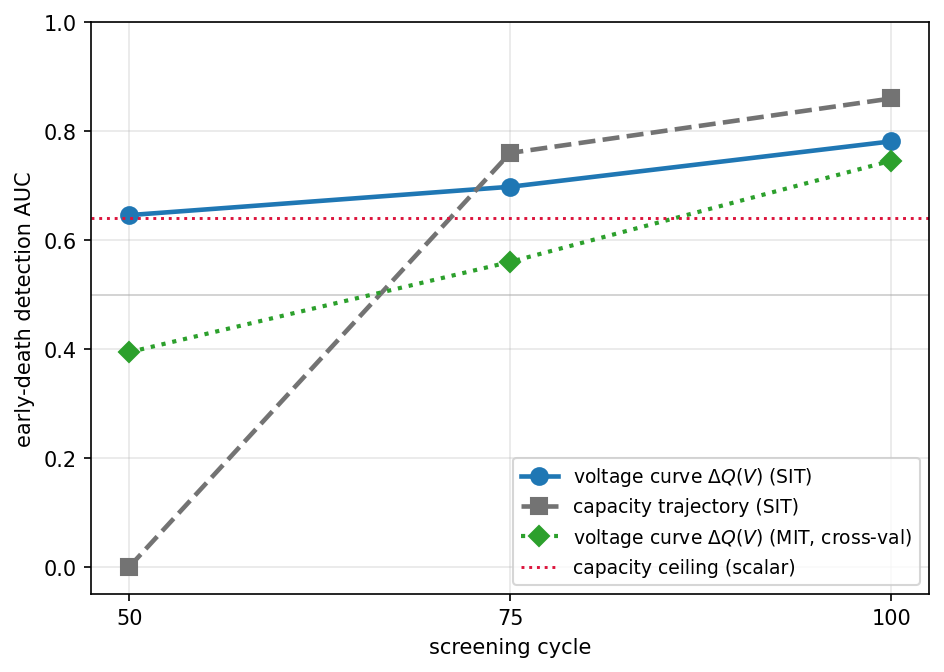
\includegraphics[width=\linewidth]{figures/fig_screening.png}
\caption{Early detection AUC versus screening cycle.}\label{fig:screen}
\end{figure}


\section{Remaining Useful Life Forecasting}\label{sec:rul}
% RUL forecasting extension. Style: hyphens in compounds are fine; no em or en dashes; short captions.
The hybrid of Section~\ref{sec:method} predicts the next-cycle SOH. For deployment the
decision-relevant quantity is the remaining useful life (RUL), defined here as the number of
cycles until a cell first reaches the 0.80 end-of-life (EOL) threshold. Converting a one-step
model into an RUL forecaster is not trivial. The natural approach is to roll the model forward
autoregressively, feeding each prediction back as the next input. We find, consistent with
recent forecasting studies~\cite{seq2seq_rul, ed_lstm}, that this recursive scheme accumulates
error over the horizon and, once a cell enters nonlinear accelerated ageing, tends to
extrapolate the last observed near-linear slope and miss the knee. On the SIT cells this
failure is severe. The recursive lineage forecasts an RUL for only 38\% to 86\% of the cells
that reach EOL, and it abstains on the very cells that matter, the fast-failing G1
cells 001-8 and 101-3 that carry the manufacturing defect.

\subsection{Direct trajectory decoding}\label{sec:rul_direct}
We extend the hybrid with a direct multi-horizon decoder that predicts the whole remaining SOH
trajectory in a single forward pass, which removes the iterative feedback and its error
accumulation~\cite{seq2seq_rul, batterymformer}. The pretrained encoder, comprising the
early-life fingerprint and the observed window, is retained unchanged. A compact decoder head
outputs the SOH at a fixed set of future horizons up to 600 cycles, and the RUL is read as the
first horizon that crosses 0.80. We keep the decoder deliberately simple. On the 20-cell target
set, richer architectures overfit and lose coverage: an encoder-decoder LSTM with attention
reaches an RUL error of 96 and 43 cycles at the 30\% and 50\% anchors with coverage 79\%, and a
transformer self-attention encoder reaches 95 and 72 cycles, whereas the compact decoder reaches
68 and 49 cycles at full coverage. This is consistent with reports that simpler models dominate
when target data are scarce~\cite{cnn_robust}.

\subsection{Foundation pretraining}\label{sec:rul_foundation}
Because the target set is small, transfer is decisive. We extend the single-source pretraining
of the base hybrid into a multi-dataset LFP foundation corpus of 155 cells drawn from the MIT,
HUST, and SNL collections, and we pretrain the trajectory decoder on this corpus before
leave-one-cell-out fine-tuning on the SIT cells. This is the largest single lever we found.
Table~\ref{tab:rul} reports a clear ablation ladder. Training from scratch gives 182 and 102
cycles of error at the 30\% and 50\% anchors, MIT-only pretraining gives 85 and 100, and the
155-cell foundation corpus gives 68 and 49. Foundation pretraining also repairs calibration. The
from-scratch model is overconfident, with prediction interval coverage of 9\% to 40\%, whereas
the foundation model attains 82\% to 100\%.

\subsection{Probabilistic RUL}\label{sec:rul_prob}
We propagate the Monte Carlo Dropout ensemble through the trajectory to obtain a predictive RUL
distribution, and we report the median together with an 80\% interval calibrated by
leave-one-out conformal inference~\cite{conformal_rul}. The calibrated intervals attain 80\%
empirical coverage, and at the 50\% anchor the median width tightens from 285 to 175 cycles
relative to the raw ensemble. At the 30\% anchor the intervals remain wide, which honestly
reflects the intrinsic difficulty of forecasting a thirteenfold spread in end-of-life from
early data.

\subsection{Forecasting Accuracy and Coverage}\label{sec:rul_results}
Table~\ref{tab:rul} and Figure~\ref{fig:rul} summarise the comparison against the recursive
lineage; errors are in cycles, and a blank prediction-interval-coverage entry marks methods
that produce no intervals. The foundation model forecasts every cell that reaches EOL, including the two
catastrophic cells the recursive methods cannot, at a median error of 68 and 49 cycles and with
calibrated intervals. The recursive DE-LSTM attains a lower error, 41 and 12 cycles, but only on
the easy 38\% to 86\% of cells that it chooses to forecast. This is the coverage against risk
trade-off familiar from selective prediction~\cite{reject_option}. A method that withholds a
forecast on the defective cells is of limited use for a manufacturing screen, where those cells
are precisely the ones of interest. The direct decoder also reduces the error of the
autoregressive hybrid from 98 to 68 cycles at the earliest anchor.

\begin{table}[t]
\centering
\caption{RUL forecasting on the SIT cells.}\label{tab:rul}
\footnotesize
\setlength{\tabcolsep}{4pt}
\begin{tabular}{llccc}
\hline
Anchor & Method & Cov. & Med.\ err. & PI cov. \\
\hline
30\% & Hybrid, foundation & 100\% & 68 & 82\% \\
     & \quad abl.\ MIT only & 100\% & 85 & \\
     & \quad abl.\ from scratch & 100\% & 182 & 9 to 40\% \\
     & DE-LSTM, recursive & 38\% & 41 & \\
     & GA-LSTM, recursive & 38\% & 78 & \\
     & Hybrid, recursive & 62\% & 98 & \\
\hline
50\% & Hybrid, foundation & 100\% & 49 & 90\% \\
     & \quad abl.\ MIT only & 100\% & 100 & \\
     & DE-LSTM, recursive & 86\% & 12 & \\
     & Hybrid, recursive & 86\% & 11 & \\
\hline
\end{tabular}
\end{table}

\begin{figure*}[t]
\centering
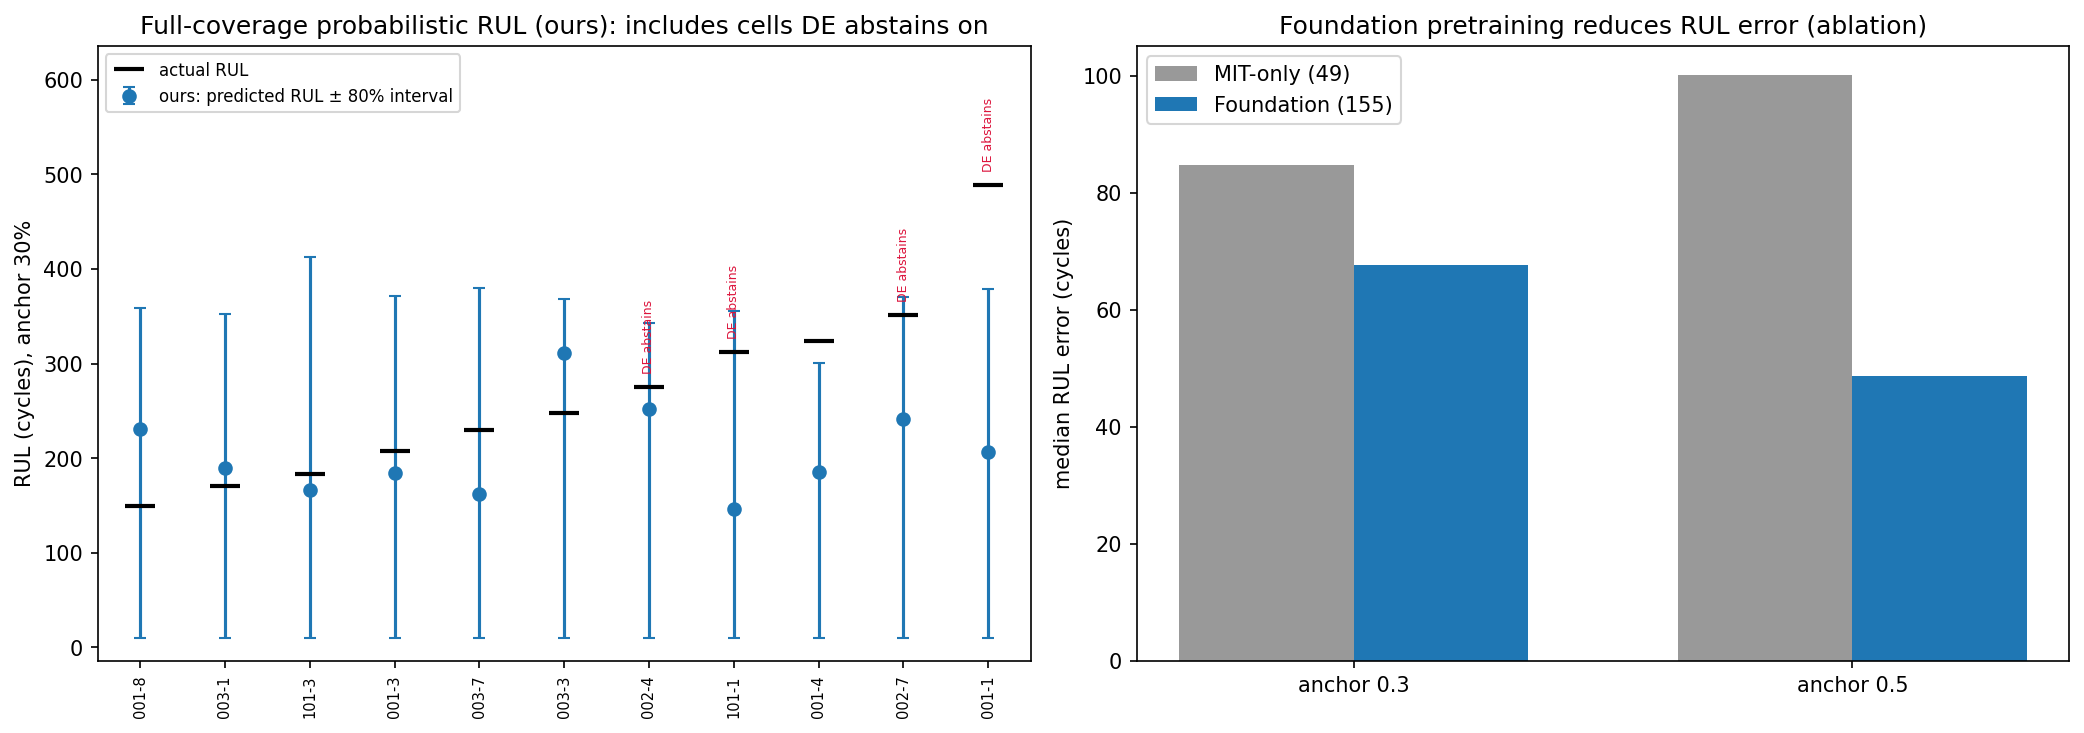
\includegraphics[width=0.9\textwidth]{figures/fig_rul_benchmark.png}
\caption{Full-coverage probabilistic RUL and the pretraining ablation.}\label{fig:rul}
\end{figure*}


\section{Discussion}\label{sec:discussion}
This section interprets the results for deployment, covering manufacturing
variability, the saturation of the standard one-step benchmark, the chemistry
alignment principle, the complementary roles of the early-life fingerprint and
fine tuning, pretraining-run variance and reproducibility, and the model's
computational footprint, before setting out the study's limitations.

\subsection{Manufacturing Variability as the Primary Bottleneck}

The central lesson of the SIT data is that prediction error lives in the cell,
not the algorithm: within-cell trajectories are highly predictable, yet
nominally identical cells diverge so widely (Section~\ref{sec:variability}) that
cell identity, not the choice of method, sets the error floor
(Section~\ref{sec:baseline}). The field's effort, dominated by architectural
innovation, is thus allocated against where the variance actually lies. For a
BMS engineer the practical consequence is an asymmetric risk: same-cell models
underestimate catastrophic degraders, while naive cross-cell pooling degrades
ordinary robust cells; the fingerprint encoder is our response, conditioning
each prediction on the cell's own early-life behaviour before any fine tuning
begins. The same variability also explains why benchmarks built on hand-picked,
smoothly degrading cells are systematically optimistic, and why a dataset that
spans catastrophic to exceptionally robust cells is a more honest proving
ground.

\subsection{Benchmark Saturation: A Floor Check, Not a Leaderboard}

The most consequential methodological finding is that rolling one-step-ahead
prediction is saturated on these smooth trajectories: a trivial 20-cycle linear
autoregressor matches or beats every deep model, and inter-method gaps fall
within the run-to-run variance of training itself (Section~\ref{sec:baseline}).
The obvious harder alternative, recursive multi-step rollout, discriminates no
better here, since feeding predictions back accumulates error until every model
is unusable. One-step RMSE is therefore a floor check, not a leaderboard. We
accordingly recommend that studies on smooth-degradation data (i)~always include
a trivial persistence or linear baseline, (ii)~report multi-run variance under
deterministic seeding, and (iii)~rank methods on the capabilities the
application needs, early-life prediction, calibrated uncertainty, and
cross-chemistry robustness, rather than on fourth-decimal RMSE. The same
discipline applies across operating conditions: apparent temperature-transfer
effects here reflect test-set difficulty rather than easy transfer, and must be
controlled for (Section~\ref{sec:brittleness}).

\subsection{The Chemistry Alignment Principle}

Uncertainty calibration transferred only when the pretraining and deployment
chemistries matched (Section~\ref{sec:cross_dataset}). The mechanism is simple:
the model's learned sense of how uncertain to be is tuned to LFP degradation
dynamics, so its intervals are appropriately scaled on LFP cells but
overconfident on the faster-fading LCO cells. The practical rule is to pretrain
on chemistry-matched data. Because even matched intervals under-cover, we regard
split-conformal correction (or temperature scaling~\cite{guo2017calibration})
as mandatory before prediction intervals are trusted in a BMS, whether or not
the chemistry is matched.

\subsection{Fingerprint and Fine Tuning: Distinct Roles, Not Rivals}

The ablation and its shuffled-fingerprint control together show that the
fingerprint's role is to anchor the LSTM in the pretrained population's regime
rather than to identify the individual cell, a weaker mechanism than we first
hypothesised but a more robust one, since it needs only a representative
pretraining population, not 30 cycles rich enough to tell cells apart. The
cross-dataset experiment then separates the two levers by role: fine tuning is
the \emph{dependable} mechanism, positive in every transfer scenario including
each cross-chemistry pair, whereas zero-shot fingerprint conditioning is the
\emph{early-life} mechanism, the only option before any history exists and most
reliable exactly when chemistry and corpus breadth match, the setting a
manufacturer qualifying a product line can guarantee. For a BMS this means a
chemistry-matched model is useful from the first cycles at no adaptation cost,
with fine tuning taking over as history accumulates and becoming indispensable
once chemistries differ.

\subsection{Pretraining-Run Variance and Reproducibility}

A surprising hazard is how strongly transfer quality depends on the pretraining
draw, and that no source-domain metric we tested identified the poorly
transferring runs (Section~\ref{sec:selection}); one-step holdout RMSE was in
fact inverted, rewarding collapsed persistence-like solutions. Any transfer
pipeline whose pretraining objective admits a trivial shortcut may share this
silent failure mode, which single-run studies cannot detect; our
calibration-cell protocol is a deployable safeguard, and we recommend that
battery-prognostics transfer studies report multi-run variance. The companion
discipline is determinism: every number in this paper reproduces byte-for-byte
from a fresh clone (Section~\ref{sec:repro}), a practice we adopted after finding
that library-default seeding alone could alter experimental conclusions.

\subsection{Computational Footprint}

A recurring justification for this work is BMS deployment, which constrains model
size and inference cost, so we report both.
The hybrid is lightweight: 21\,089 parameters, approximately 82\,KB in float32
and 41\,KB in float16, small enough to reside in the memory of an embedded BMS
microcontroller.
A point SOH estimate is a single forward pass; the 50-pass MC-Dropout
uncertainty estimate, when the passes are evaluated as one batched forward
(replicating the input across the batch dimension), completes in about 4\,ms on
both a desktop CPU and the RTX 2080 Ti.
Because SOH is updated once per charge-discharge cycle (tens of minutes to
hours), this leaves a latency margin of several orders of magnitude; even an
unoptimised implementation that runs the 50 passes sequentially
($\approx$1\,s) would be comfortably within budget.
These figures were measured on a desktop CPU rather than production embedded
silicon, so absolute timings would differ on a microcontroller; nonetheless the
41\,KB footprint and few-millisecond batched inference indicate the model fits
well within the resource envelope of contemporary BMS hardware.

\subsection{Limitations}

The findings reported above should be read alongside the boundaries of the
present study. The limitations listed below stem mainly from dataset scale and
the scope of the experimental design rather than from the hybrid framework
itself, and each points to a concrete opportunity for future work: larger cell
cohorts would sharpen the statistical claims, shorter fingerprint windows and
format-matched pretraining data would broaden applicability, and post hoc
calibration would close the residual coverage gap. We state them explicitly so
that practitioners can judge how far the present conclusions transfer to their
own deployment setting.

\begin{enumerate}
  \item \textit{G1 sample size}: With ten G1 cells, LOOCV results have limited
        statistical power. The observed two-sided pattern (pooling rescues
        catastrophic degraders and harms robust cells) is directionally
        consistent, but quantitative conclusions should be interpreted with
        this sample size in mind.

  \item \textit{Fingerprint window}: The 30-cycle fingerprint requires at least
        30 discharge cycles before cell-specific predictions are available.
        For applications requiring earlier prediction (e.g., first 10 cycles),
        shorter window studies would be needed.

  \item \textit{Residual calibration gap}: Even after split-conformal
        correction, coverage reaches 93.9\%, not the nominal 95\%, and two
        extreme cells (001-8, 003-5) remain substantially under-covered.
        Conformal guarantees assume exchangeability between calibration and
        test cells, which manufacturing outliers violate by definition;
        detecting such cells online (e.g.\ from interval-width anomalies)
        remains open.

  \item \textit{Format mismatch}: The MIT pretraining cells are 18650 cylindrical
        (1.1\,Ah); the SIT cells are 50\,Ah prismatic.
        Despite this format difference, the LFP chemistry match appears sufficient
        for meaningful transfer.
        Format-matched pretraining data would likely reduce the remaining gap further.

  \item \textit{LISHEN source corpus size}: The LISHEN dataset contributes only
        three cells to the cross-dataset evaluation (scenarios M and N).
        The consistently weak gains in these scenarios ($-$24.6\% to
        $+$14.6\% for ZS+FP) are attributed to insufficient source diversity
        rather than a fundamental limitation of the fingerprint mechanism.
        Future work should re-evaluate with a larger LISHEN corpus.

  \item \textit{Calibration-cell requirement}: The checkpoint-selection
        protocol requires three target-domain cells cycled to (or near) end of
        life. This is realistic for a manufacturer qualifying a product, but
        not for retrofitting arbitrary third-party packs; in that setting a
        chemistry-matched public dataset could serve as a weaker substitute,
        which we have not evaluated.

  \item \textit{Comparison scope}: Beyond the four LSTM-family predictors
        (Simple LSTM, PA-LSTM, GA-LSTM, DE-LSTM), we benchmarked two modern
        non-recurrent architectures (TCN, Transformer) and two trivial
        baselines under the identical protocol
        (Table~\ref{tab:method_comparison}).
        The modern baselines were run under fixed configurations rather than
        the per-cell hyperparameter search afforded to GA/PA/DE-LSTM; given
        the saturation of the one-step metric we do not expect tuning to
        change the conclusions, but other model classes (e.g.\
        Gaussian-process regression) remain for future work.

  \item \textit{Evaluation protocol}: The saturation finding implies that
        one-step RMSE, including our own accuracy numbers, has limited power
        to rank methods on these data.
        Harder protocols (fixed early-life budgets, multi-step horizons with
        scheduled sampling, knee-onset prediction) are the right arena for
        future accuracy claims; we did not re-benchmark all methods under
        such protocols here.
\end{enumerate}


\section{Conclusion}\label{sec:conclusion}
We investigated the deployment challenges for battery SOH prediction that are
absent from small-cell laboratory benchmarks, using a new 18-month dataset of 20
large-format LiFePO$_4$ prismatic cells (50\,Ah) cycled under three operating
conditions.

Its central message is that on large-format cells manufacturing variability, not
algorithm choice, dominates prediction error, and that because one-step accuracy
on their smooth trajectories saturates, models should be judged by the deployment
capabilities they add rather than by one-step rank. We therefore report trivial
baselines and multi-run variance as standard practice.

Guided by this, our hybrid model (MIT LFP pretraining, a convolutional
fingerprint encoder, and MC-Dropout uncertainty) is positioned not as the most
accurate one-step predictor but as the one that supplies what deployment needs:
prediction of a new cell from only its first 30 cycles with no target-cell
training, a substantial accuracy gain once fine tuning begins, and calibrated
uncertainty after a lightweight conformal correction. A ten-scenario
cross-dataset validation shows that fine tuning is the dependable adaptation
mechanism, that zero-shot fingerprint conditioning adds distinctive value when
chemistry and corpus match, and that uncertainty stays calibrated only under
chemistry alignment, a practical guideline for BMS transfer learning. We also
identify pretraining-run variance as a silent reproducibility hazard and
neutralise it with a calibration-cell selection protocol, in a fully
deterministic, byte-for-byte reproducible pipeline.

Building on the same model, we demonstrated two further capabilities aimed
directly at manufacturing variability: an early screen that flags defective cells
from the discharge voltage curve well before the capacity trajectory reveals
them, and a full-coverage probabilistic RUL forecaster that, through a direct
multi-horizon decoder and a 155-cell LFP foundation corpus, forecasts every cell
reaching end of life, including the catastrophic cells recursive baselines
abstain on.

Taken together, this work moves SOH and RUL prediction beyond the small-cell
laboratory setting that has dominated the field, contributing a large-format LFP
benchmark with trivial-baseline controls, evidence that the field's default
evaluation protocol needs rethinking, an uncertainty-calibrated and
deployment-oriented model validated across manufacturers, chemistries, and
operating conditions, and a fully deterministic pipeline with a released
checkpoint. Future work should pursue harder evaluation protocols on which deep
models may separate from trivial baselines, shorter fingerprint windows and
format-matched pretraining, online detection of cells that violate conformal
exchangeability, and pretraining objectives that exclude trivial shortcut
solutions.


\section*{Acknowledgements}
The authors thank the Singapore Institute of Technology Battery Laboratory
for providing the experimental infrastructure and cycling data used in this study.
The MIT dataset used for pretraining was made available by Severson et al.\
under open-access terms~\cite{severson2019data}.

\section*{Data and Code Availability Statement}
The SIT large-format LiFePO$_4$ dataset analysed in this study is openly
available at \url{https://doi.org/10.25447/sit.32101523}~\cite{ponnambalam2026sitdata}.
The MIT/Severson fast-charging dataset is openly available from Severson et
al.~\cite{severson2019data}, and the NASA dataset from the NASA Prognostics
Center of Excellence~\cite{saha2007battery}.
This study is designed to be fully reproducible. All code, the complete
experimental pipeline, and the selected pretrained checkpoint that generate every
table and figure in this paper are available at
\url{https://github.com/karthicgrepo/battery-soh-prediction}.
Every experiment runs deterministically, using TensorFlow op-determinism with full
float32 precision and complete seeding of the Python, NumPy, and TensorFlow random
number generators, so each reported value reproduces bit-for-bit on the same
hardware and software stack.

% CRediT roles below are a draft for the authors to confirm before submission.
\section*{CRediT authorship contribution statement}
\textbf{Karthickumar Ponnambalam:} Conceptualization, Methodology, Software,
Formal analysis, Investigation, Data curation, Visualization, Writing - original
draft. \textbf{Sivaneasan Balakrishnan:} Resources, Data curation, Supervision,
Writing - review and editing. \textbf{Anurag Sharma:} Supervision, Validation,
Writing - review and editing. \textbf{Sze Sing Lee:} Supervision, Writing -
review and editing.

\section*{Declaration of competing interest}
The authors declare that they have no known competing financial interests or
personal relationships that could have appeared to influence the work reported
in this paper.

\section*{Funding}
This research did not receive any specific grant from funding agencies in the
public, commercial, or not-for-profit sectors.

\section*{Declaration of generative AI and AI-assisted technologies in the writing process}
During the preparation of this work the authors used an AI-assisted coding and
writing assistant to help with code refactoring, analysis scripting, and
language editing. After using this tool, the authors reviewed and edited the
content as needed and take full responsibility for the content of the
publication.

\bibliographystyle{elsarticle-num}
\bibliography{references}

\end{document}
